% !TeX spellcheck = sp
\documentclass[a4paper,11pt]{article}
%\documentclass[a4paper,twoside,11pt,titlepage]{book}
\usepackage[utf8]{inputenc}
\usepackage[spanish]{babel}
\usepackage{tikz}
\usepackage{tikz-cd}
\usetikzlibrary{babel}
%\usepackage[round]{natbib}
\usepackage[backend=bibtex,citestyle=alphabetic]{biblatex}
\addbibresource{bibliography/bibliography.bib}
\usepackage{float}
\usepackage{tikz-3dplot}
\usepackage[toc,page]{appendix}
\usetikzlibrary{patterns}
\usetikzlibrary{calc}
\usepackage{pgfplots}
\usetikzlibrary{external}
\usepackage{amsmath,amsthm,amssymb}
\usepackage{caption}
\usepackage{subcaption}

\usepackage{hyperref}
\usepackage{xcolor}

\hypersetup{
    colorlinks,
    citecolor=black,
    filecolor=black,
    linkcolor=black,
    urlcolor=black
}

\setlength{\parindent}{2em}
\setlength{\parskip}{0.4em}
\renewcommand{\baselinestretch}{1.0}
\setlength{\textfloatsep}{5pt}

\usepackage{minted}
\definecolor{monokaibg}{HTML}{272822}
\definecolor{friendlybg}{HTML}{f0f0f0}

% \usepackage[style=list, number=none]{glossary} %
%\usepackage{titlesec}
%\usepackage{pailatino}

\graphicspath{{img/}}
\decimalpoint
\usepackage{dcolumn}
\newcolumntype{.}{D{.}{\esperiod}{-1}}
\makeatletter
\addto\shorthandsspanish{\let\esperiod\es@period@code}
\makeatother


%\usepackage[chapter]{algorithm}
\RequirePackage{verbatim}
%\RequirePackage[Glenn]{fncychap}
\usepackage{fancyhdr}
\usepackage{graphicx}
\usepackage{afterpage}

\usepackage{longtable}
 
% ********************************************************************
% Re-usable information
% ********************************************************************
\newcommand{\myTitle}{P3-Navarro-Ramírez-Pilar.pdf\xspace}
\newcommand{\myDegree}{Grado en Ingeniería Informática y Matemáticas\xspace}
\newcommand{\myName}{Pilar Navarro Ramírez\xspace}
%\newcommand{\myProf}{M. Jesús García-Ligero Ramírez\xspace}
%\newcommand{\myOtherProf}{Carlos Ureña Almagro\xspace}
\newcommand{\myFaculty}{Escuela Técnica Superior de Ingenierías Informática y de
Telecomunicación\xspace}
\newcommand{\myFacultyShort}{E.T.S. de Ingenierías Informática y de
Telecomunicación\xspace}
\newcommand{\myUni}{\protect{Universidad de Granada}\xspace}
\newcommand{\myLocation}{Granada\xspace}
\newcommand{\myTime}{\today\xspace}
\newcommand{\myVersion}{Version 0.1\xspace}

\hypersetup{
pdfauthor = {\myName antoniogamiz10@gmail.com},
pdftitle = {\myTitle},
pdfsubject = {},
pdfkeywords = {raytracing, montecarlo, random, numbers},
pdfcreator = {pdflatex},
pdfproducer = {pdflatex}
}

%\hyphenation{}


%\usepackage{doxygen/doxygen}
\usepackage{url}
\usepackage{colortbl,longtable}
\usepackage[stable]{footmisc}
%\usepackage{index}

%\makeindex
%\usepackage[style=long, cols=2,border=plain,toc=true,number=none]{glossary}
% \makeglossary

% Definición de comandos que me son tiles:
%\renewcommand{\indexname}{Índice alfabético}
%\renewcommand{\glossaryname}{Glosario}

\pagestyle{fancy}
\fancyhf{}
\fancyhead[LO]{\leftmark}
\fancyhead[RE]{\rightmark}
\fancyhead[RO,LE]{\textbf{\thepage}}
%\renewcommand{\chaptermark}[1]{\markboth{\textbf{#1}}{}}
%\renewcommand{\sectionmark}[1]{\markright{\textbf{\thesection. #1}}}

\setlength{\headheight}{1.5\headheight}

\newcommand{\HRule}{\rule{\linewidth}{0.5mm}}
%Definimos los tipos teorema, ejemplo y definición podremos usar estos tipos
%simplemente poniendo \begin{teorema} \end{teorema} ...
%\newtheorem{theorem}{Teorema}[chapter]
%\newtheorem{example}{Ejemplo}[chapter]
%\newtheorem{definition}[chapter]{Definición}

\newcommand{\bigrule}{\titlerule[0.5mm]}


%Para conseguir que en las páginas en blanco no ponga cabecerass
\makeatletter
\def\clearpage{%
  \ifvmode
    \ifnum \@dbltopnum =\m@ne
      \ifdim \pagetotal <\topskip
        \hbox{}
      \fi
    \fi
  \fi
  \newpage
  \thispagestyle{empty}
  \write\m@ne{}
  \vbox{}
  \penalty -\@Mi
}
\makeatother

\usepackage{pdfpages}

\usepackage[a4paper, margin={1in}]{geometry}

\begin{document}

\begin{titlepage}
 
 
\newlength{\centeroffset}
\setlength{\centeroffset}{-0.5\oddsidemargin}
\addtolength{\centeroffset}{0.5\evensidemargin}
\thispagestyle{empty}

\noindent\hspace*{\centeroffset}\begin{minipage}{\textwidth}

\centering

\includegraphics[width=0.9\textwidth]{img/logo_ugr.jpg}\\[2cm]

\textsc{ \Huge Inteligencia de Negocio\\[1.5cm]}
\textbf{\textsc{ \huge Práctica 3:}}\\
 \huge  Competición en Kaggle\\[1cm]
% Upper part of the page
% 
% Title
%{\Huge\bfseries \\
%}
%\noindent\rule[-1ex]{\textwidth}{3pt}\\[3.5ex]
%{\large\bfseries }
\end{minipage}

\vspace{2cm}
\noindent\hspace*{\centeroffset}\begin{minipage}{\textwidth}
\centering

\textbf{Autor}\\[0.2cm] {Pilar Navarro Ramírez}\\[0.2cm]
pilarnavarro@correo.ugr.es \\[0.2cm]
Grupo de prácticas 1 \\[1cm]


\includegraphics[width=0.3\textwidth]{img/etsiit_logo.png}\\[0.1cm]
\textsc{Escuela Técnica Superior de Ingeniería Informática y de Telecomunicaciones}\\
\textsc{---}\\
Granada, 4 de enero de 2021
\end{minipage}
%\addtolength{\textwidth}{\centeroffset}
%\vspace{\stretch{2}}
\end{titlepage}



%\input{preface/preface}

%\tableofcontents
%\listoffigures
%\listoftables

\newpage

\begin{figure}[H]
	\centering
	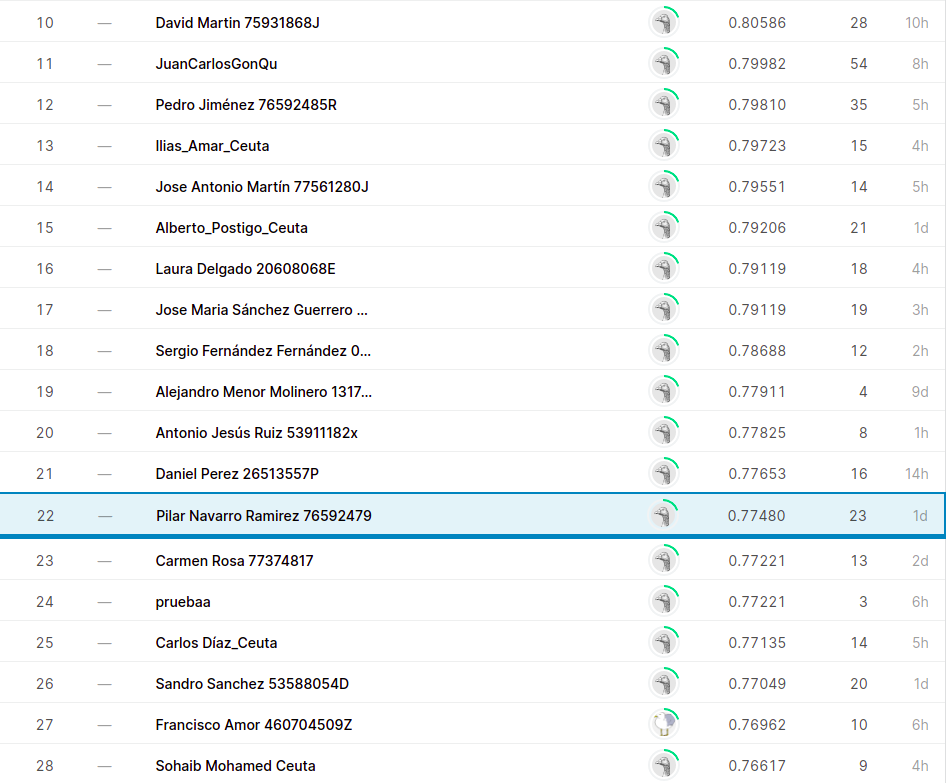
\includegraphics[width=1\linewidth]{img/resultados}
	\caption{}
	\label{fig:resultados}
\end{figure}
\newpage
\tableofcontents

\newpage
\section{Entrega 1}
\subsection{Preprocesamiento}
En esta primera entrega tomamos un primer contacto con el conjunto de datos de entrenamiento y test del que disponemos. Para ello, una vez cargados ambos conjuntos como DataFrames de pandas, obtenemos información de los mismos haciendo uso de la función \mintinline{python}{info()}, con la que obtenemos las siguientes salidas:

\begin{figure}[H]
	\centering
	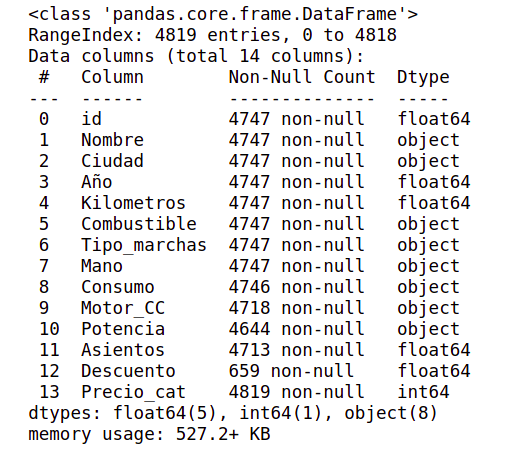
\includegraphics[width=0.5\linewidth]{img/train}
	\caption{Conjunto de entrenamiento}
	\label{fig:train}
\end{figure}

\begin{figure}[H]
	\centering
	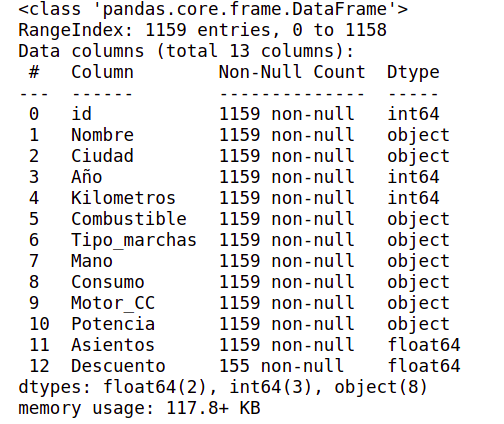
\includegraphics[width=0.5\linewidth]{img/test}
	\caption{Conjunto de test}
	\label{fig:test}
\end{figure}


Podemos observar que hay muchos datos nulos en el conjunto de entrenamiento, por lo que procedemos a intentar deshacernos de ellos. Pero antes eliminamos la columna del \textit{id} en ambos conjuntos de datos, pues no aporta información para la clasificación sino que nos lleva directamente a un sobreajuste.  Nos damos cuenta, haciendo uso del método \mintinline{python}{describe()} sobre el conjunto de entrenamiento,

\begin{figure}[H]
	\centering
	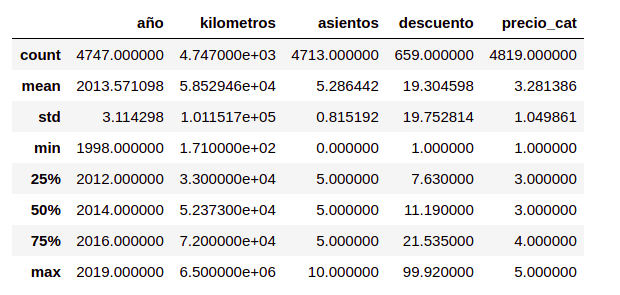
\includegraphics[width=0.8\linewidth]{img/train2}
	\caption{}
	\label{fig:train2}
\end{figure}

 que los \textit{asientos} son 5 en una gran parte de los datos de que disponemos, puesto que la media es $5.286$ y el 25,50 y 75\% de los datos tienen un valor de 5 para los asientos. Así pues, si reemplazamos los nulos de esta columna por el valor más frecuente, no perjudicaríamos demasiado los datos. Y esto es lo que hacemos utilizando el \mintinline{python}{SimpleImputer} de sklearn:
\begin{minted}{python}
imputer=impute.SimpleImputer(strategy="most_frequent")
values = imputer.fit_transform([df_train.asientos.values])
df_train.asientos.update(pd.Series(values[0]))
\end{minted}

Por otro lado, cabe notar que la columna de \textit{descuentos} es prácticamente nula, de manera que nos aporta muy poca información y la mejor opción sería eliminarla. La borramos pues tanto del conjunto de entrenamiento como del de test. Finalmente, eliminamos directamente el resto de valores nulos  del conjunto de entrenamiento con la función \mintinline{python}{dropna()} y separamos los datos en los atributos que vamos a usar para el entrenamiento y el atributo a predecir, obteniendo así los DataFrame \mintinline{python}{df_train} y \mintinline{python}{df_train_obj} respectivamente. 

A continuación, tratamos con las variables categóricas, esto es, las convertimos a variables numéricas utilizando \mintinline{python}{LabelEnconder}, tanto en el conjunto de entrenamiento como en el de test: 
\begin{minted}{python}
categorical=["nombre","ciudad","combustible","tipo_marchas",
		"mano","consumo","motor_cc","potencia"]

df_train_num=df_train.copy()
df_test_num=df_test.copy()

for atributo in categorical:
	data=pd.read_csv("data/"+atributo+".csv")
	data.columns = [col.lower() for col in data]
	label = LabelEncoder().fit(data[atributo])
	df_train_num[atributo]=label.transform(df_train[atributo])
	df_test_num[atributo]=label.transform(df_test[atributo])
\end{minted}

Cabe mencionar que hemos usado los archivos \textit{atributo.csv} para convertir los valores categóricos a numéricos, de manera que cada categoría sea consistente con el valor numérico asociado en el conjunto de entrenamiento y el de test. Como resultado de este proceso obtenemos los DataFrame \mintinline{python}{df_train_num} y \mintinline{python}{df_test_num}.

Por último, normalizamos todos los datos numéricos en el intervalo $[0,1]$. Para ello utilizamos \mintinline{python}{MinMaxScaler} de sklearn aplicado a cada uno de los archivos \textit{atributo.csv}, de manera que el máximo y mínimo considerados para la normalización sean los adecuados al rango de valores que toma cada atributo. Obtenemos así los conjuntos de datos \mintinline{python}{df_train_norm} y \mintinline{python}{df_test_norm}. El código usado para llevar esto a cabo ha sido el siguiente: 
\begin{minted}{python}
cols = [col for col in df_train_orig.columns if col not in ['precio_cat','id','descuento']]  
categorical=["nombre","ciudad","combustible","tipo_marchas",
			"mano","consumo","motor_cc","potencia"]

df_train_norm=df_train_num.copy()
df_test_norm=df_test_num.copy()


for atributo in cols:
	data=pd.read_csv("data/"+atributo+".csv")
	data.columns = [col.lower() for col in data]
	if atributo in categorical:
		label = LabelEncoder().fit(data[atributo])
		data[atributo]=label.transform(data[atributo])
	scaler = MinMaxScaler().fit(data.values)
	train_values=df_train_num[atributo].values.reshape(-1,1)
	df_train_norm[atributo]=scaler.transform(train_values)
	test_values=df_test_num[atributo].values.reshape(-1,1)
	df_test_norm[atributo]=scaler.transform(test_values)
\end{minted}

\subsection{Aplicación de los algoritmos}

Una vez llevado a cabo todo el preprocesamiento mencionado procedemos a aplicar algunos clasificadores usando \textbf{Cross Validation} con 5 folds. Para realizar la validación cruzada hacemos uso de la función \mintinline{python}{cross_val_score} con la medida de accuracy, que nos devuelve un vector con los valores de la precisión obtenidos en cada una de las particiones, al que le calculamos la media para obtener una medida de la calidad del clasificador sobre el conjunto de entrenamiento. Definimos así la siguiente función, que usaremos de aquí en adelante: 
\begin{minted}{python}
def cross_validation(clf,x,y,mostrar=False):
	scores=cross_val_score(clf,x,y,scoring='accuracy',cv=5)
	accuracy=np.mean(scores)  
	if mostrar:
		print("Accuracy: ", accuracy)
	return accuracy
\end{minted}

Entrenamos entonces usando esta función una máquina de soporte vectorial lineal, un árbol de decisión, un Random Forest, una Red neuronal y el algoritmo de los vecinos más cercanos, dejando a todos estos modelos los parámetros por defecto, y los resultados obtenidos para la precisión con cada uno de ellos han sido los siguientes:
\begin{figure}[H]
	\centering
	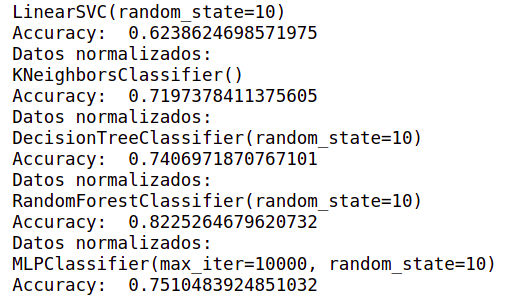
\includegraphics[width=0.5\linewidth]{img/alg1}
	\caption{}
	\label{fig:alg1}
\end{figure}

Podemos observar que el que ofrece un valor más prometedor es el Random Forest, por lo que vamos a entrenar dicho modelo con todos los datos de entrenamiento preprocesados y aplicarlo al conjunto de test para realizar una primera subida a Kaggle:
\begin{minted}{python}
forest=RandomForestClassifier(random_state=10)
forest.fit(df_train_norm,df_train_obj)
pred=forest.predict(df_test_norm)
ids=df_test_orig["id"]

df_result = pd.DataFrame({'id': ids, 'Precio_cat': pred})
df_result.to_csv("resultados_1.csv", index=False)
\end{minted}

\subsection{Características entrega}
Las características de esta subida han sido las siguientes: 

\begin{table}[htbp]
	\caption{}
	\begin{tabular}{|c|c|c|c|}
		\hline
		\textbf{} & \textbf{} & \multicolumn{ 2}{c|}{\textbf{Score}} \\ \hline
		\textbf{Fecha y Hora} & \textbf{Posición en Ranking (hasta ese momento)} & \textbf{Train} & \textbf{Test} \\ \hline
		23 de diciembre 21:30 & 10 & 0.822526 & 0.74374 \\ \hline
	\end{tabular}
	\label{}
\end{table}



\section{Entrega 2}
\subsection{Preprocesamiento}
En este caso hemos cambiado ligeramente el tratamiento realizadao a los datos nulos. En concreto, puesto que al reemplazar los asientos nulos por el valor más frecuente de su columna podemos estar introduciendo información falsa, en esta segunda prueba hemos decidido elimiar tambińe directamente los valores nulos de los asientos. Sin embargo, trabajamos en paralelo con los dos preprocesamientos, llamando \mintinline{python}{df_train_replaced} y \mintinline{python}{df_train_obj_replaced} a los datos de entrenamiento y a sus correspondientes etiquetas respectivamente donde los asientos nulos han sido reemplazados por la moda, y \mintinline{python}{df_train} y  \mintinline{python}{df_train_obj} a los datos y etiquetas donde todos los nulos han sido eliminados. 
En este punto, ambos conjuntos de datos, junto con el conjunto de test, reciben el mismo preprocesamiento realizado en la entrega anterior, a saber, paso de variables categóricas a numéricas con LabelEncoder, y normalización de los datos en el intervalo $[0,1]$
\subsection{Aplicación de los algoritmos}

Usamos ahora la función \mintinline{python}{cross_validation}, cuya implementación ya hemos explicado, para medir la calidad de los algoritmos aplicados sobre cada uno de los dos datos de entrenamiento preprocesados considerados:
\begin{table}[htbp]
	\caption{}\begin{center}
	
	\begin{tabular}{|c|c|c|l|}
		\hline
		\multicolumn{ 2}{|c|}{\textbf{Nulos reemplazados en asientos}} & \multicolumn{ 2}{c|}{\textbf{Nulos eliminados}} \\ \hline
		LinearSVC & 0.6238624698 & 0.62734051186 &  \\ \hline
		Knn & 0.719737841 & 0.735815543 &  \\ \hline
		RandomForest & 0.740697187 & 0.743059925 &  \\ \hline
		DecisionTree & 0.8225264679 & 0.8227918227 &  \\ \hline
		Red Neuronal & 0.7510483924 & 0.6995602372 &  \\ \hline
	\end{tabular}\end{center}
	\label{}
\end{table}

Podemos observar que en todos los algoritmos los resultados son ligeramente superiores con todos los nulos eliminados, salvo en las redes neuronales, lo cual es lógico pues estas necesitan bastantes datos para poder ser bien entrenada, por lo que si disponen de más datos el resultado que producen es mejor. 
\subsection{Configuración de los parámetros}
Como el algoritmo de Random Forest es el que nos ha dado los mejores resultados, nos centramos en configurar los parámetros del mismo y usando los datos en que eliminamos todos los nulos, pues han resultado ser mejores, como ya hemos comprobado. 

Para la configuración usamos varias funciones, cada una de ellas centrada en el ajuste de un parámetro concreto, las cuales iteran sobre un determinado rango de valores y almacenan los resultados obtenidos al aplicar la función \mintinline{python}{cross_validation} al clasificador con un valor del parámetro diferente en cada iteración. Los resultados del accuracy almacenados se muestran finalmente en una gráfica, con la que podemos entonces determinar qué valor del parámetro es el más apropiado.
El código usado en cada caso con sus correspondientes gráficas resultantes son los siguientes: 
 \begin{minted}{python}
 #Para el parámetro min_samples_split
 def tune_forest_1(max_value):
	 acc=[]
	 for i in range(2,max_value):
		 forest=RandomForestClassifier(min_samples_split=i,random_state=10)
		 acc.append(cross_validation(forest,df_train_norm,df_train_obj))
		 
	 fig, ax =plt.subplots(figsize=(15,5))
	 ax.plot(range(2,max_value), acc)
	 ax.set_title('Random Forest')
	 ax.set_xlabel('Valor parámetro')
	 ax.set_ylabel('Accuracy')
	 plt.show()
 \end{minted}
 
 \begin{figure}[H]
 	\centering
 	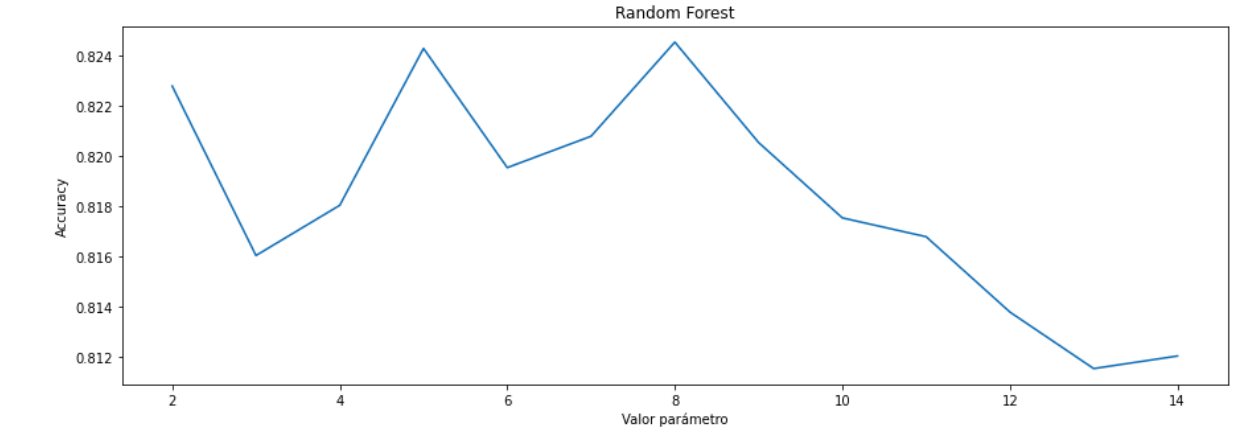
\includegraphics[width=0.7\linewidth]{img/forest1}
 	\caption{}
 	\label{fig:forest1}
 \end{figure}
 
 \begin{minted}{python}
 #Para el parámetro max_depth
 def tune_forest_2(max_value):
	 acc=[]
	 for i in range(2,max_value):
		 forest=RandomForestClassifier(max_depth=i,random_state=10)
		 acc.append(cross_validation(forest,df_train_norm,df_train_obj))
	 
	 fig, ax =plt.subplots(figsize=(15,5))
	 ax.plot(range(2,max_value), acc)
	 ax.set_title('Random Forest')
	 ax.set_xlabel('Valor parámetro')
	 ax.set_ylabel('Accuracy')
	 plt.show()
 \end{minted}
 \begin{figure}[H]
 	\centering
 	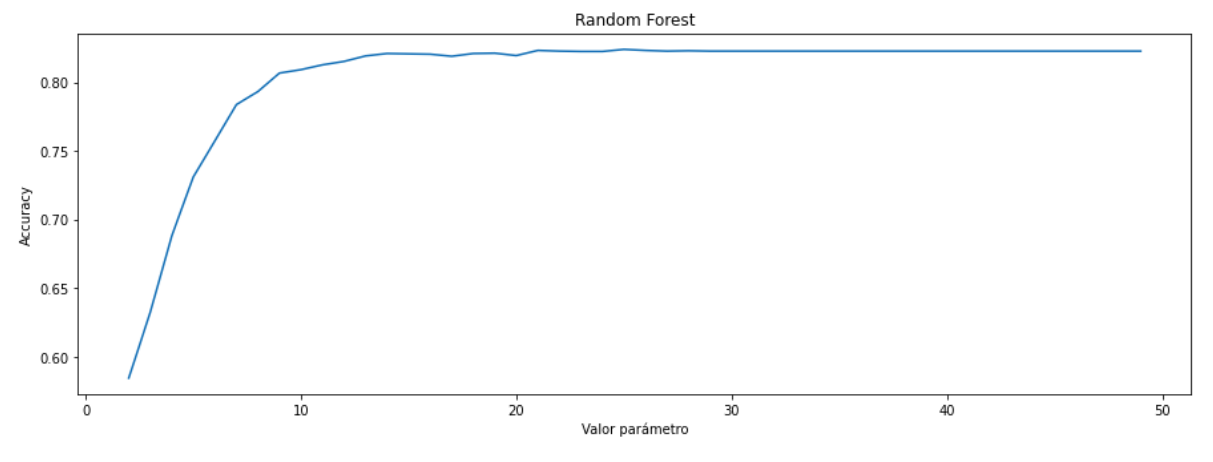
\includegraphics[width=0.7\linewidth]{img/forest2}
 	\caption{}
 	\label{fig:forest2}
 \end{figure}
 
 \begin{minted}{python}
#Para el parámetro max_leaf_nodes
def tune_forest_3(max_value):
	acc=[]
	for i in range(2,max_value):
		forest=RandomForestClassifier(max_leaf_nodes=i,random_state=10)
		acc.append(cross_validation(forest,df_train_norm,df_train_obj))
		
	fig, ax =plt.subplots(figsize=(15,5))
	ax.plot(range(2,max_value), acc)
	ax.set_title('Random Forest')
	ax.set_xlabel('Valor parámetro')
	ax.set_ylabel('Accuracy')
	plt.show()
 \end{minted}

 \begin{figure}[H]
 	\centering
 	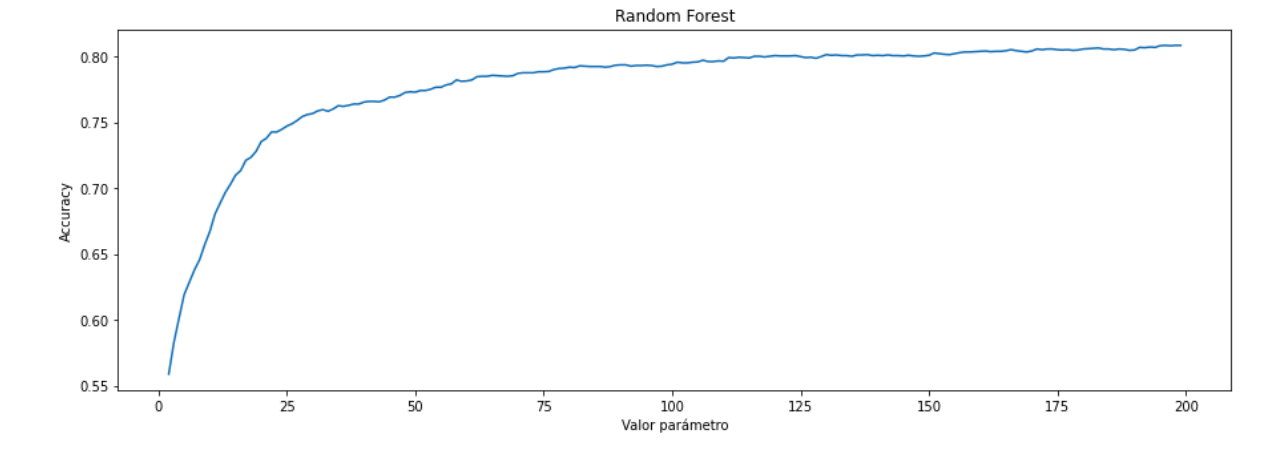
\includegraphics[width=0.7\linewidth]{img/forest3}
 	\caption{}
 	\label{fig:forest3}
 \end{figure}
 
\begin{minted}{python}
#Para el parámetro min_samples_leaf
def tune_forest_4(max_value):
	acc=[]
	for i in range(2,max_value):
		forest=RandomForestClassifier(min_samples_leaf=i,random_state=10)
		acc.append(cross_validation(forest,df_train_norm,df_train_obj))
	
	fig, ax =plt.subplots(figsize=(15,5))
	ax.plot(range(2,max_value), acc)
	ax.set_title('Random Forest')
	ax.set_xlabel('Valor parámetro')
	ax.set_ylabel('Accuracy')
	plt.show()
\end{minted}
\begin{figure}[H]
	\centering
	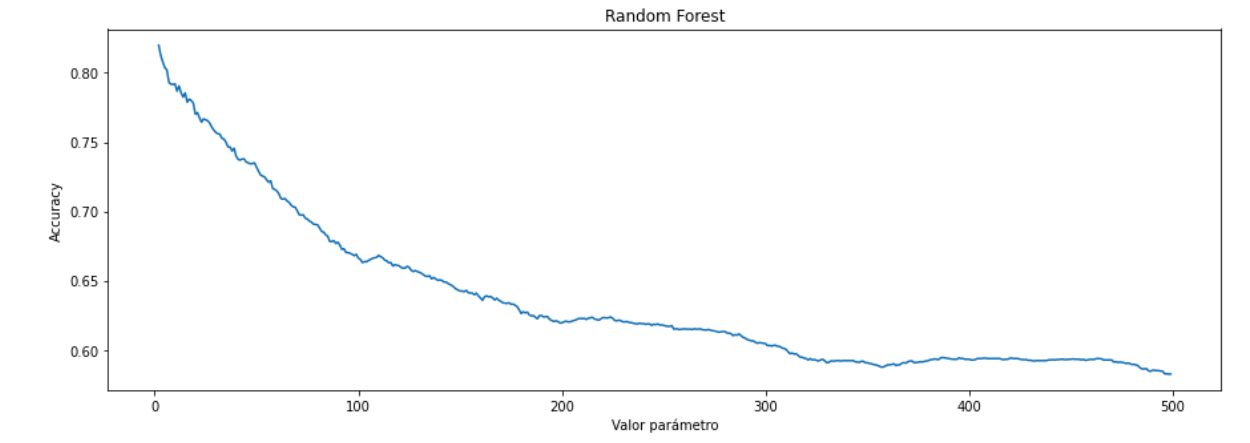
\includegraphics[width=0.7\linewidth]{img/forest4}
	\caption{}
	\label{fig:forest4}
\end{figure}

\begin{minted}{python}
#Para el parámetro n_estimators
def tune_forest_5(max_value):
	acc=[]
	for i in range(2,max_value):
		forest=RandomForestClassifier(n_estimators=i,min_samples_split=8,
									random_state=10)
		acc.append(cross_validation(forest,df_train_norm,df_train_obj))
	
	fig, ax =plt.subplots(figsize=(15,5))
	ax.plot(range(2,max_value), acc)
	ax.set_title('Random Forest')
	ax.set_xlabel('Valor parámetro')
	ax.set_ylabel('Accuracy')
	plt.show()
	tune_forest_5(400)
\end{minted}
\begin{figure}[H]
	\centering
	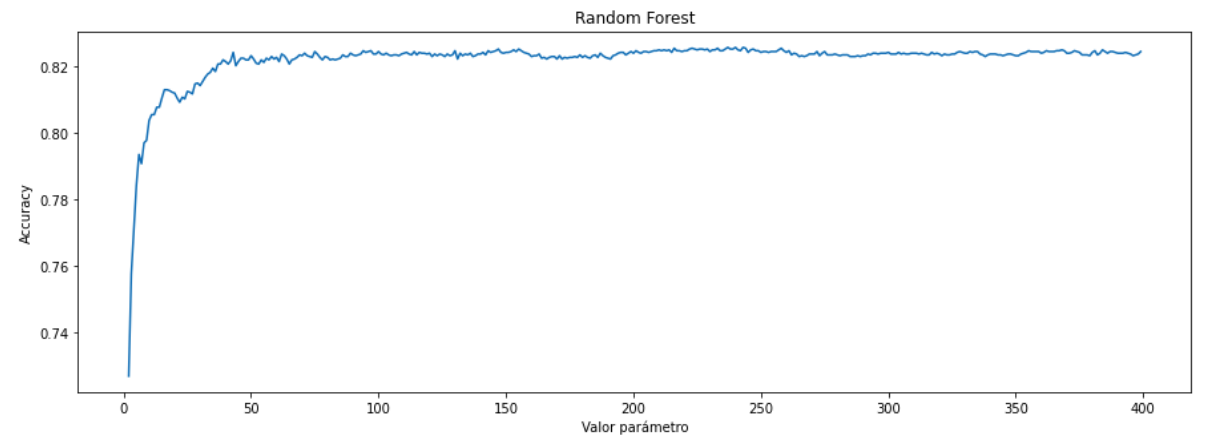
\includegraphics[width=0.7\linewidth]{img/forst5}
	\caption{}
	\label{fig:forst5}
\end{figure}

Se puede apreciar entonces que, salvo para el parámetro \mintinline{python}{min_samples_split}, para los demás parámetros los resultados no mejoran al cambiar sus valores por defecto, sino que en la mayoría de los casos empeoran o se mantienen igual. Es más, probando algunos de los valores para los que en las gráficas se ven con mejores resultados, hemos obtenido unos resultados peores. Sin embargo, si fijamos el parámetro \mintinline{python}{min_samples_split} a un valor de 8, sí que obtenemos un valor mayor de la precisión que el que obtenemos con ese parámetro por defecto. En concreto, obtenemos 
\begin{minted}{python}
Accuracy:  0.8245411
\end{minted}

que es mejor al de por defecto: 

\begin{minted}{python}
Accuracy:  0.8227918
\end{minted}

Así pues, con este preprocesamiento realizado a los datos, y los parámetros por defecto salvo \mintinline{python}{min_samples_split=8}, procedemos a realizar una segunda entrega, realizando una clasificación de los datos de test con RandomForest configurado como lo indicado:

\begin{minted}{python}
forest=RandomForestClassifier(n_estimators=100,min_samples_split=8,random_state=10)
forest.fit(df_train_norm,df_train_obj)
pred=forest.predict(df_test_norm)
ids=df_test_orig["id"]

df_result = pd.DataFrame({'id': ids, 'Precio_cat': pred})
df_result.to_csv("resultados_2.csv", index=False)
\end{minted}

\subsection{Características de la entrega}

\begin{table}[htbp]
	\caption{}\begin{center}
	\begin{tabular}{|c|c|c|c|c|}
		\hline
		\multicolumn{1}{|l|}{} & \textbf{} & \textbf{} & \multicolumn{ 2}{c|}{\textbf{Score}} \\ \hline
		\textbf{Entrega} & \textbf{Fecha y Hora} & \textbf{Posición en Ranking (hasta ese momento)} & \textbf{Train} & \textbf{Test} \\ \hline
		\textbf{1} & 23 de diciembre 21:30 & 10 & 0.822526 & 0.74374 \\ \hline
		\textbf{2} &  24 de diciembre  16:51 & 10 & 0.8245411 & 0.74029 \\ \hline
	\end{tabular}\end{center}
	\label{}
\end{table}


Observamos que los resultados obtenidos con los parámetros configurados de Random Forest han sido ligeramente inferiores a los obtenidos en la entrega anterior, con Random Forest con parámetros por defecto, de manera que a partir de ahora trabajamos con este con sus parámetros por defecto. 
\section{Entrega 3}
\subsection{Preprocesamiento}

Llevamos a cabo el mismo preprocesamiento realizado en la entrega anterior: eliminación de todos los nulos o reemplazamiento de los nulos en asientos por la moda, transformación de variables categóricas a numéricas con LabelEncoder y normalización.

\subsection{Aplicación de los algoritmos}

En esta ocasión nos centramos en otros clasificadores que nos ofrece \mintinline{python}{sklearn.ensemble}, a parte de RandomForest. Vamos a estudiar Gradient Boosting, AdaBoost, clasificador de Extra-Trees y Bagging con el algoritmo de vecinos más cercanos. 

Ejecutamos pues la función \mintinline{python}{cross_validation} con cada uno de ellos y con los dos conjuntos de datos que obtenemos de los dos preprocesamientos diferentes realizados, obteniendo los siguientes valores de la precisión:

\begin{table}[htbp]
	\caption{}\begin{center}
	\begin{tabular}{|c|c|c|}
		\hline
		\multicolumn{ 2}{|c|}{\textbf{Nulos reemplazados en asientos}} & \textbf{Nulos eliminados} \\ \hline
		Knn & 0.719737841 & 0.735815543 \\ \hline
		Bagging con Knn & 0.763619383720153 & 0.780305867665418 \\ \hline
		Extra-Trees & \multicolumn{1}{r|}{0.813159269405283} & \multicolumn{1}{r|}{0.807795880149813} \\ \hline
		RandomForest & 0.8225264679 & 0.8227918227 \\ \hline
		AdaBoost & 0.604655202784375 & 0.675589575530587 \\ \hline
		Gradient Boosting & 0.805523194013351 & \multicolumn{1}{r|}{0.806548064918851} \\ \hline
	\end{tabular}\end{center}
	\label{}
\end{table}

Podemos observar que, como con los clasificadores vistos en la entrega anterior, los resultados son mejores para casi todos ellos cuando eliminamos todos los valores nulos, de manera que vamos a trabajar con este conjunto de datos. El algoritmo de AdaBoost es el que nos ofrece los peores valores de la precisión y, de nuevo, Random Forest es el mejor. Cabe mencionar que haciendo Bagging del algoritmo de los vecinos más cercanos, los resultados mejoran significativamente con respecto a los que nos ofrece uno solo de los clasificadores de K-nn.

\subsection{Configuración de los parámetros}

En esta entrega nos vamos a centrar en configurar los parámetros del clasificador de Bagging con Knn como estimador base, pues ya hemos visto que nos ofrece buenos resultados, los cuales pueden mejorar aún más si elegimos los valores adecuados de los parámetros. 
\subsubsection{Knn}
Para empezar, analizamos con qué número de vecinos trabaja mejor el algoritmo de K-nn con nuestros datos. Para ello usamos la siguiente función:

\begin{minted}{python}
def tune_knn(max_value):
	acc=[]
	for i in range(2,max_value):
		knn=KNeighborsClassifier(n_neighbors=i)
		acc.append(cross_validation(knn,df_train_norm,df_train_obj))
	
	fig, ax =plt.subplots(figsize=(15,5))
	ax.plot(range(2,max_value), acc)
	ax.set_title('Vecino más cercano')
	ax.set_xlabel('Num vecinos')
	ax.set_ylabel('Accuracy')
	plt.show()
\end{minted} 
que, como las usadas en la entrega anterior para configurar los parámetros del Random Forest, itera sobre un rango de valores para el número de vecinos, almacena la precisión obtenida con cada uno de los valores del parámetros y muesta finalmente una gráfica con los resultados.
\begin{figure}[H]
	\centering
	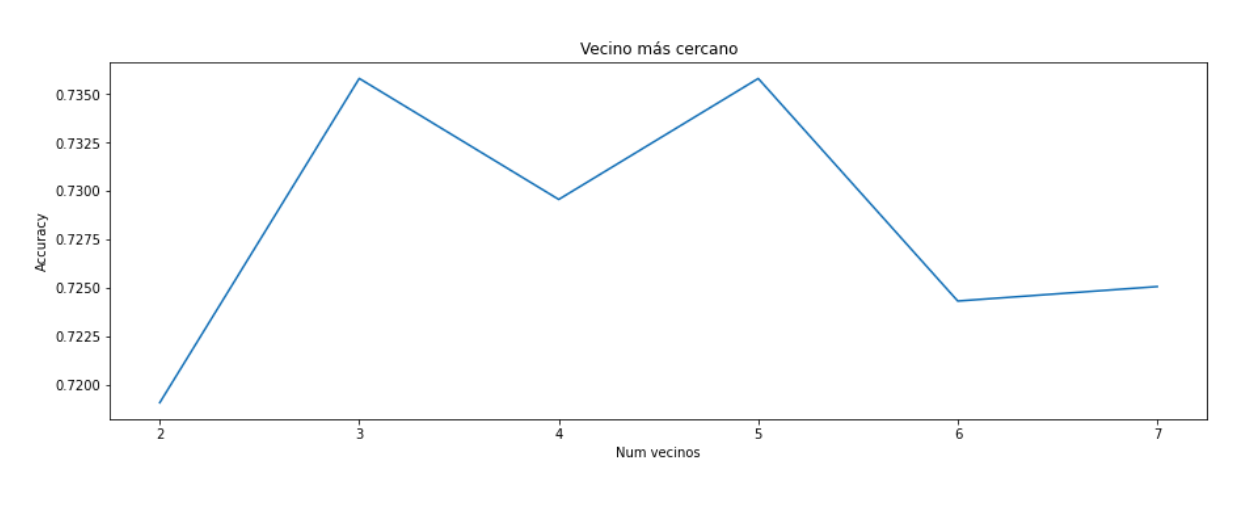
\includegraphics[width=0.8\linewidth]{img/knn}
	\caption{}
	\label{fig:knn}
\end{figure}

Así, los mejores resultados se obtienen para un número de vecinos de 5, que es el valor por defecto. 
\subsubsection{Bagging}
 De este algoritmo, configuramos el parámetro \mintinline{python}{max_samples}(fracción del conjunto de datos a usar para entrenar cada uno de los estimadores, con reemplazamiento), \mintinline{python}{max_features} (fracción de los atributos a usar para entrenar cada estimador base, sin reemplazamiento) y el número de estimadores (\mintinline{python}{n_estimators}). 
 
 Para \mintinline{python}{max_samples} y \mintinline{python}{max_features} probamos con algunos valores a mano y vemos los resultados: 
 
 \begin{figure}[H]
 	\centering
 	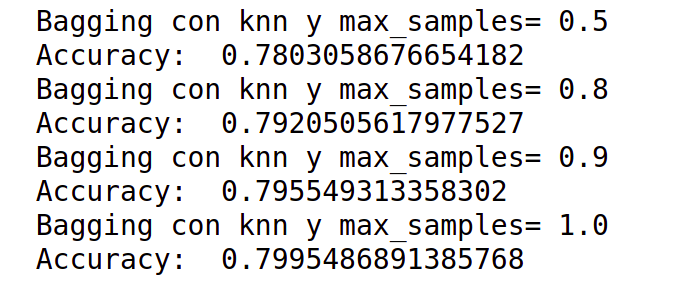
\includegraphics[width=0.5\linewidth]{img/bagging1}
 	\caption{\mintinline{python}{max_samples}  }
 	\label{fig:bagging1}
 \end{figure}
 
 \begin{figure}[H]
 	\centering
 	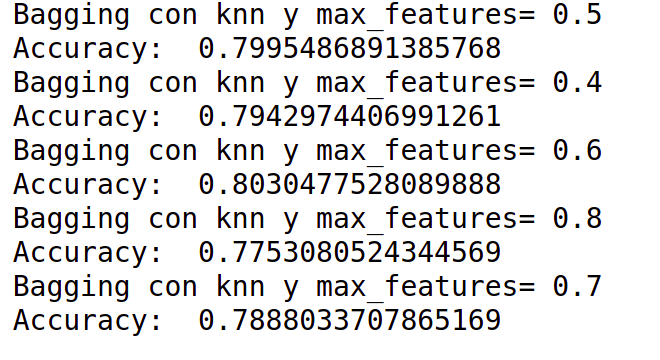
\includegraphics[width=0.5\linewidth]{img/bagging2}
 	\caption{\mintinline{python}{max_features}}
 	\label{fig:bagging2}
 \end{figure}
 
 de manera que la mejor configuración es \mintinline{python}{max_samples=1.0, max_features=0.6}.
 
 Para configurar el número de estimadores, usamos una función como las que venimos usando hasta ahora:
 
 \begin{minted}{python}
 def tune_bagging_knn(max_value):
	 acc=[]
	 for i in range(2,max_value):
		 bagging_knn= BaggingClassifier(knn,n_estimators=i, max_samples=1.0,
		 				max_features=0.6, random_state=10)
		 acc.append(cross_validation(bagging_knn,df_train_norm,df_train_obj))
	 
	 fig, ax =plt.subplots(figsize=(15,5))
	 ax.plot(range(2,max_value), acc)
	 ax.set_title('Bagging con knn')
	 ax.set_xlabel('Num estimadores')
	 ax.set_ylabel('Accuracy')
	 plt.show()
 \end{minted}
 
 que muestra la siguiente salida si le proporcionamos un \mintinline{python}{max_value} de 40:
 
 \begin{figure}[H]
 	\centering
 	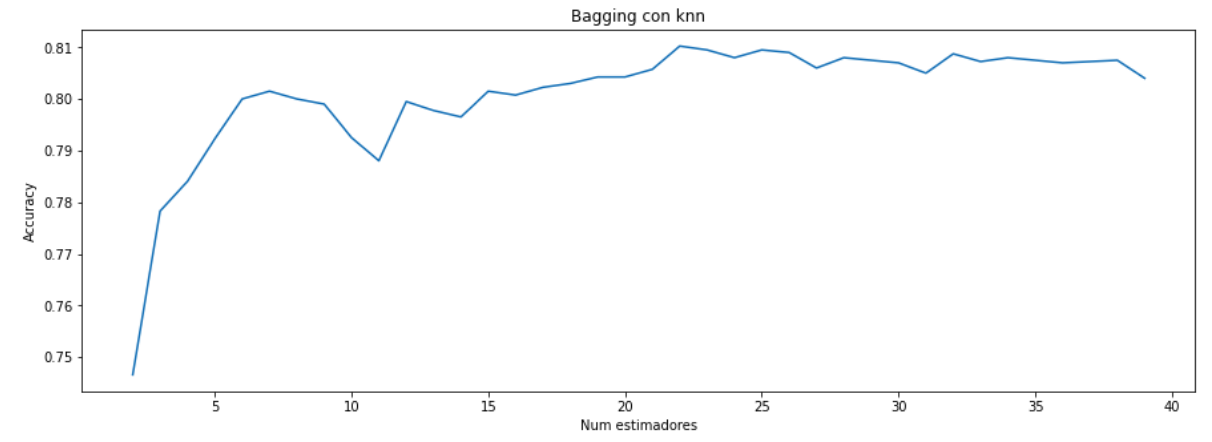
\includegraphics[width=0.8\linewidth]{img/bagging3}
 	\caption{}
 	\label{fig:bagging3}
 \end{figure}
 
 de manera que la mayor precisión se obtiene con un número de estimadores de 22. 
 
 Por lo tanto, si aplicamos sobre el conjunto de entrenamiento (preprocesado con todos los nulos eliminados) el clasificador de Bagging con Knn como estimador base, con la mejor configuración de parámetros obtenida, el valor de la precisión aplicando cross-validation con 5 particiones es el siguiente:
 \begin{minted}{python}
 Accuracy:  0.8102943196004995
 \end{minted}

 Llevamos a cabo la clasificación del conjunto de test preprocesado como en las entregas anteriores, usando el clasificador de Bagging con Knn y los parámetros ya especificados, y subimos los resultados a Kaggle. 
 
 \begin{minted}{python}
 knn=KNeighborsClassifier()
 bagging_knn= BaggingClassifier(knn,n_estimators=22, max_samples=1.0,
  max_features=0.6, random_state=10)
 bagging_knn.fit(df_train_norm,df_train_obj)
 pred=bagging_knn.predict(df_test_norm)
 ids=df_test_orig["id"]
 
 df_result = pd.DataFrame({'id': ids, 'Precio_cat': pred})
 df_result.to_csv("resultados_3.csv", index=False)
 \end{minted}
 
 \subsection{Características de la entrega}

 \begin{table}[htbp]
 	\caption{}
 	\begin{tabular}{|c|c|c|c|c|}
 		\hline
 		\multicolumn{1}{|l|}{} & \textbf{} & \textbf{} & \multicolumn{ 2}{c|}{\textbf{Score}} \\ \hline
 		\textbf{Entrega} & \textbf{Fecha y Hora} & \textbf{Posición en Ranking (hasta ese momento)} & \textbf{Train} & \textbf{Test} \\ \hline
 		\textbf{3} & 24  de dic iembre19:49 & 13 & 0.8102943 & 0.72389 \\ \hline
 	\end{tabular}
 	\label{}
 \end{table}
 
 \section{Entrega 4}
 Para esta entrega partimos de los mismos datos que en la anterior y nos centramos en configurar los parámetros del algoritmo de \textbf{Gradient Boosting} (el código se encuenta en el mismo notebook que la entrega 3, \mintinline{python}{p3_3.ipynb})
 \subsection{Configuración de los parámetros}
 Fijamos el valor del parámetro \mintinline{python}{max_features} a 'auto', de manera que se considera un número de atributos igual a la raíz cuadrada del número total de atributos para buscar la mejor partición en cada caso, y empezamos estudiando el parámetro subsample, que determina la fracción de los datos proporcionados a usar para entrenar a cada árbol base. 
 
 Tras probar con algunos valores aleatorios, en concreto con $0.6,0.8,0.7,0.9$, obtenemos los mejores resultados con $subsample=0.7$, que nos ofrece \mintinline{python}{Accuracy:  0.8118005617977527}. 
 
 El siguiente paso es configurar el máximo de profundidad que puede llegar a tomar cada uno de los árboles, para lo cual hacemos uso de la siguiente funcion:
 \begin{minted}{python}
 def tune_gradient_boosting(max_value):
	 acc=[]
	 for i in range(1,max_value):
		 gradient=GradientBoostingClassifier(max_depth=i,
		 random_state=10,subsample=0.7)
		 acc.append(cross_validation(gradient,df_train_norm,df_train_obj))
	 
	 fig, ax =plt.subplots(figsize=(15,5))
	 ax.plot(range(1,max_value), acc)
	 ax.set_title('Gradient Boosting')
	 ax.set_xlabel('Max depth')
	 ax.set_ylabel('Accuracy')
	 plt.show()
 \end{minted}
 cuyo funcionamiento es similar al explicado en otras ocasiones para funciones con el mismo propósito. Si le proporcionamos un parámetro de 20, nos ofrece la siguiente salida: 
 \begin{figure}[H]
 	\centering
 	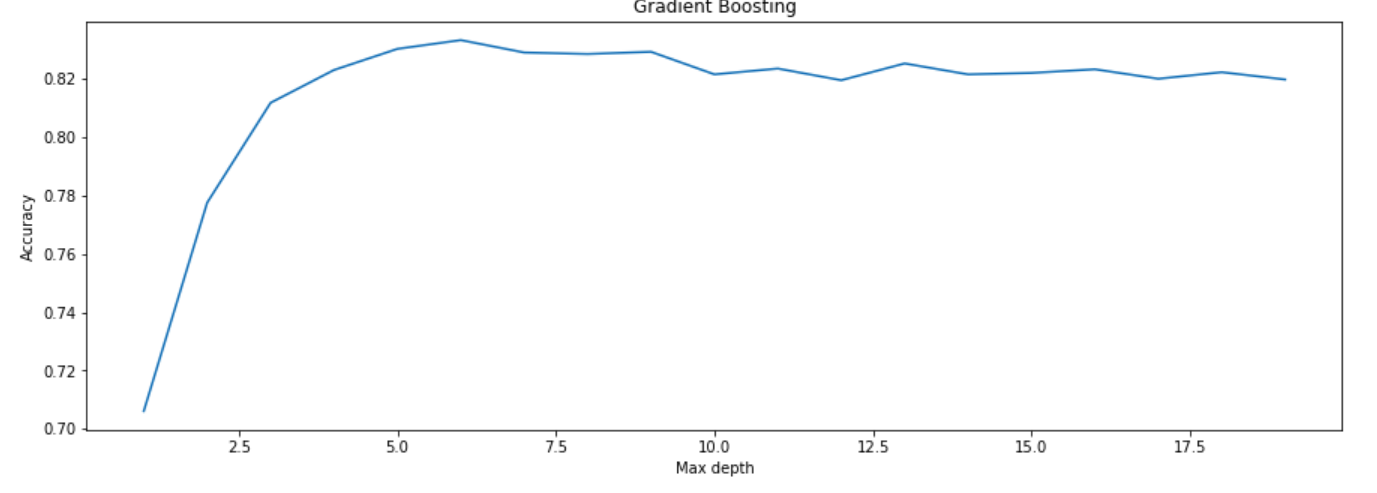
\includegraphics[width=0.7\linewidth]{img/gradient1}
 	\caption{}
 	\label{fig:gradient1}
 \end{figure}
 
 y para un máximo de 8:
 \begin{figure}[H]
 	\centering
 	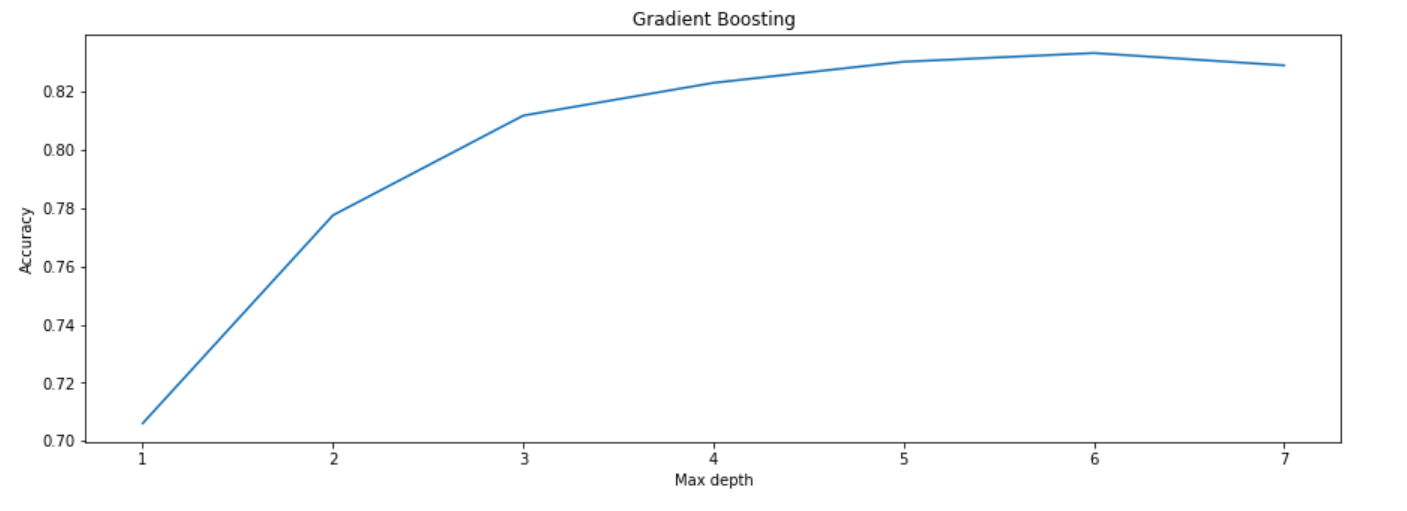
\includegraphics[width=0.7\linewidth]{img/gradient2}
 	\caption{}
 	\label{fig:gradient2}
 \end{figure}
 
 de manera que \mintinline{python}{max_depth=6} es el mejor valor para este parámetro. 
 
 Buscamos ahora el número de estimadores más adecuado, probando con ciertos valores (a saber, $300,200,100,50$) obteniendo los mejores resultados con un total de 100 estimadores: \mintinline{python}{Accuracy:  0.8332890137328339}.
 
 Finalmente estudiamos el parámetro \mintinline{python}{learning_rate} de la misma forma, probando con algunos valores aleatorios ($0.2,0.3,0.5,0.15,0.25$), siendo 0.2 el más adecuado: \mintinline{python}{Accuracy: 0.832040}
 
 Sin embargo, al probar con otras combinaciones de valores, nos damos cuenta de que los resultados son mejores: 
 \begin{minted}{python}
gradient=GradientBoostingClassifier(n_estimators=150, learning_rate=0.2, 
random_state=10,max_features='auto',subsample=0.9,max_depth=5)
cross_validation(gradient,df_train_norm,df_train_obj,True)

Accuracy:  0.8347896379525593
 \end{minted}

por lo que llevamos a cabo un Grid Search con los valores más prometedores:
\begin{minted}{python}
gradient=GradientBoostingClassifier(random_state=10,max_features='auto')
parameter_space = {
'n_estimators': [100,150,200,250],
'learning_rate': [0.2,0.1,0.3],
'subsample': [0.9, 0.7,0.6,0.8],
'max_depth':[5,6],
}

clf=GridSearchCV(gradient, parameter_space, n_jobs=-1, cv=5)
clf.fit(df_train_norm,df_train_obj)

print('Mejores parámetros: ', clf.best_params_)

Mejores parámetros:  {'learning_rate': 0.1, 'max_depth': 5, 'n_estimators': 100,
 'subsample': 0.8}
\end{minted} 
 
 que de hecho mejoran la precisión obtenida hasta ahora:
 
\mintinline{python}{Accuracy:  0.8360374531835205}
 
 Así pues, usamos esta configuración de parámetros en el clasificador, lo aplicamos al conjunto de test preprocesado y lo subimos a Kaggle.
 
 \subsection{Características de la subida}
 \begin{table}[htbp]
 	\caption{}\begin{center}
 	\begin{tabular}{|c|c|c|c|c|}
 		\hline
 		\multicolumn{1}{|l|}{} & \textbf{} & \textbf{} & \multicolumn{ 2}{c|}{\textbf{Score}} \\ \hline
 		\textbf{Entrega} & \textbf{Fecha y Hora} & \textbf{Posición en Ranking (hasta ese momento)} & \textbf{Train} & \textbf{Test} \\ \hline
 		\textbf{3} & 24  de diciembre 19:49 & 13 & 0.8102943 & 0.72389 \\ \hline
 		\textbf{4} & 24 de diciembre 21:00  & 7 & 0.836037 & 0.76704 \\ \hline
 	\end{tabular}
 	\label{}\end{center}
 \end{table}
 
 con lo que este algoritmo nos proporciona los mejores resultados hasta el momento. 
 
 \section{Entrega 5}
 \subsection{Preprocesamiento}
 El preprocesamiento será el mismo que hemos realizado en las entregas anteriores, y nos quedamos con los datos de entrenamiento en los que eliminamos todas las instancias nulas. Nos centramos aquí en el clasificador de Extra-Trees, que también proporcionaba un valor de la precisión prometedor. 
 \subsection{Configuración de parámetros}
 
 Para comenzar, activamos la opción de bootstrap, pues nos ofrece mejores resultados, y estudiamos el parámetro \mintinline{python}{max_samples}, que indica la fracción del conjunto de datos que se va a usar en el clasificador para entrenar a cada estimador base. Como hicimos en ocasiones anteriores, probamos distintos valores aleatorios ($0.9,0.8,0.7,0.5,0.95,0.87$), obteniendo los mejores resultados con \mintinline{python}{max_samples=0.9}: \mintinline{python}{Accuracy:  0.8117952559300875}.
 
 A continuación, usando la siguiente función:
 \begin{minted}{python}
 def tune_num_arboles(max_value):
	 acc=[]
	 for i in range(5,max_value,10):
		 extra=ExtraTreesClassifier(n_estimators=i,random_state=10,
		 bootstrap=True, max_samples=0.9)
		 acc.append(cross_validation(extra,df_train_norm,df_train_obj))
	 
	 fig, ax =plt.subplots(figsize=(15,5))
	 ax.plot(range(5,max_value,10), acc)
	 ax.set_title('Extra trees')
	 ax.set_xlabel('Num árboles')
	 ax.set_ylabel('Accuracy')
	 plt.show()
 \end{minted}
 con un \mintinline{python}{max_value=3000} obtenemos:
 \begin{figure}[H]
 	\centering
 	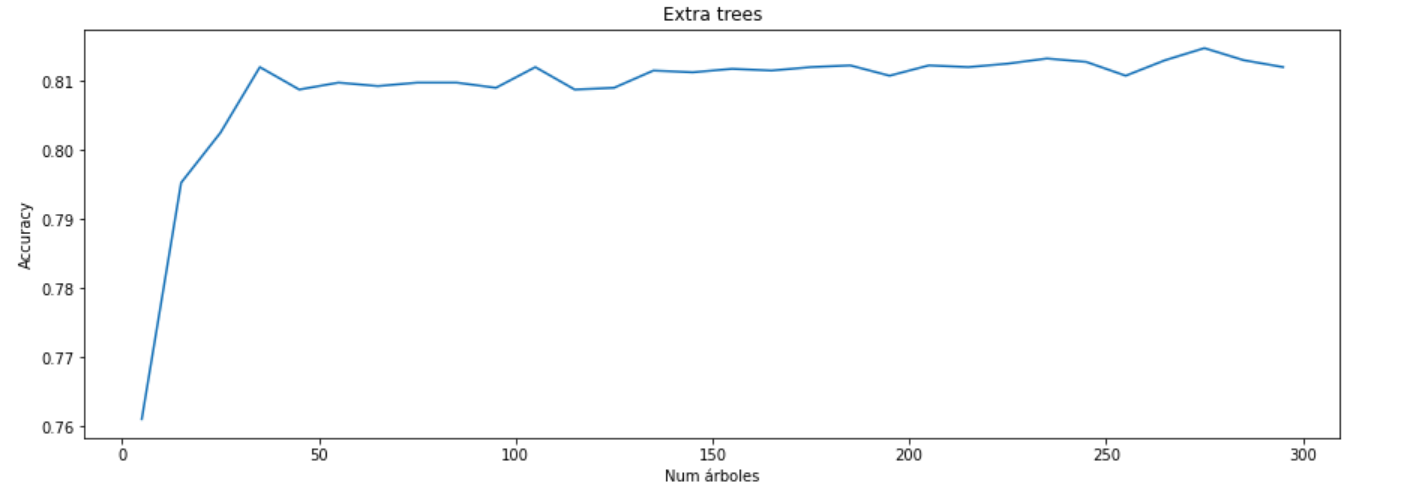
\includegraphics[width=0.9\linewidth]{img/extra1}
 	\caption{}
 	\label{fig:extra1}
 \end{figure}
 
 de manera que el número de árboles para el que los resultados son mejores es $275$:
 \begin{minted}{python}
extra=ExtraTreesClassifier(n_estimators=275,random_state=10,
bootstrap=True, max_samples=0.9)
cross_validation(extra, df_train_norm, df_train_obj,True)

Accuracy:  0.8147927590511861
 \end{minted}
 
 Para configurar la profundidad máxima de cada estimador, usamos una función igual a la anterior pero cambiando el parámetro considerado:
 
 \begin{minted}{python}
 def tune_max_depth(max_value):
	 acc=[]
	 for i in range(2,max_value):
		 extra=ExtraTreesClassifier(n_estimators=275,random_state=10,
		 bootstrap=True, max_samples=0.9,max_depth=i)
		 acc.append(cross_validation(extra,df_train_norm,df_train_obj))
		 
	 fig, ax =plt.subplots(figsize=(15,5))
	 ax.plot(range(2,max_value), acc)
	 ax.set_title('Extra trees')
	 ax.set_xlabel('Max depth')
	 ax.set_ylabel('Accuracy')
	 plt.show()
 \end{minted}
 pero no nos es de gran ayuda pues en la salida:
 \begin{figure}[H]
 	\centering
 	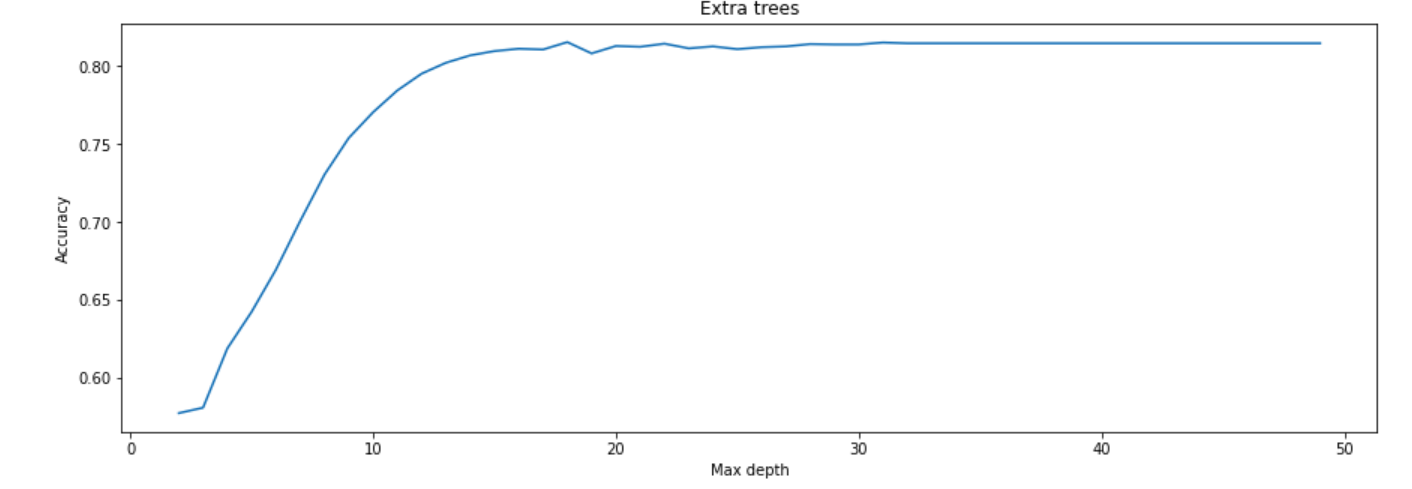
\includegraphics[width=0.9\linewidth]{img/extra2}
 	\caption{}
 	\label{fig:extra2}
 \end{figure}
 
 podemos observar que los resultados mejoran conforme aumenta la profundidad máxima, de manera que si esta no está fijada a ningún valor concreto los resultados serán mejores. Por lo tanto, dejamos el valor de \mintinline{python}{max_depth} por defecto. 
 
 Así pues, la mejor configuración de parámetros obtenida es:
 \mint{python}{n_estimators=275,bootstrap=True,max_samples=0.9}
 
 Usamos entonces el clasificador de Extra-Trees con estos parámetros entrenado sobre el conjunto de entrenamiento preprocesado como ya hemos indicado para clasificar el conjunto de test también preprocesado como en las entregas anteriores. 
 
 \subsection{Características de la entrega}
\begin{table}[htbp]
	\caption{}\begin{center}
	\begin{tabular}{|c|c|c|c|c|}
		\hline
		\multicolumn{1}{|l|}{\textbf{}} & \textbf{} & \textbf{} & \multicolumn{ 2}{c|}{\textbf{Score}} \\ \hline
		\textbf{Entrega} & \textbf{Fecha y Hora} & \textbf{Posición en Ranking (hasta ese momento)} & \textbf{Train} & \textbf{Test} \\ \hline
		\textbf{1} & 23 de diciembre 21:30 & 10 & 0.822526 & 0.74374 \\ \hline
		\textbf{2} &  24 de diciembre  16:51 & 10 & 0.8245411 & 0.74029 \\ \hline
		\textbf{3} & 24  de diciembre 19:49 & 13 & 0.8102943 & 0.72389 \\ \hline
		\textbf{4} & 24 de diciembre 21:00  & 7 & 0.836037 & 0.76704 \\ \hline
		\textbf{5} &  25 de diciembre 13:07 & 7 & 0.8147927 & 0.73856 \\ \hline
	\end{tabular}\end{center}
	\label{}
\end{table}
 Así, el resultado obtenido en Kaggle es algo menor que en los demás intentos, pero no es el peor. 
 
 \section{Entrega 6}
 \subsection{Preprocesamiento}
El preprocesamiento es igual al realizado en las entregas anteriores, usando en este caso también los datos de entrenamiento en los que eliminamos todas las instancias nulas. Estudiamos ahora las Redes Neuronales. A pesar de que este preprocesamiento ofrece resultados algo peores en las redes neuronales, nos vamos a quedar con él para intentar mejorar los resultados al configurar dichas redes, pues nos hará falta usar este clasificador con dicho preprocesamiento más adelante.  
\subsection{Configuración de parámetros}
Empezamos analizando la configuración de capas más adecuada en nuestro caso. Para ello vamos a comenzar considerando dos capas con el mismo número de nodos en cada una de ellas e implementamos una función que itere sobre dicho número y nos muestre los valores de la precisión obtenidos en cada iteración:
\begin{minted}{python}
from matplotlib import pyplot as plt
from sklearn.neural_network import MLPClassifier

def tune_layers(max_value):
	acc=[]
	for i in range(40,max_value,20):
		NN=MLPClassifier(hidden_layer_sizes=(i,i),random_state=10,max_iter=1000)
		acc.append(cross_validation(NN,df_train_norm,df_train_obj))
	
	fig, ax =plt.subplots(figsize=(15,5))
	ax.plot(range(40,max_value,20), acc)
	ax.set_title('Neural Network')
	ax.set_xlabel('Tamaño capas')
	ax.set_ylabel('Accuracy')
	plt.show()
\end{minted}
Si ejecutamos esta función con un \mintinline{python}{max_value=600} obtenemos:
\begin{figure}[H]
	\centering
	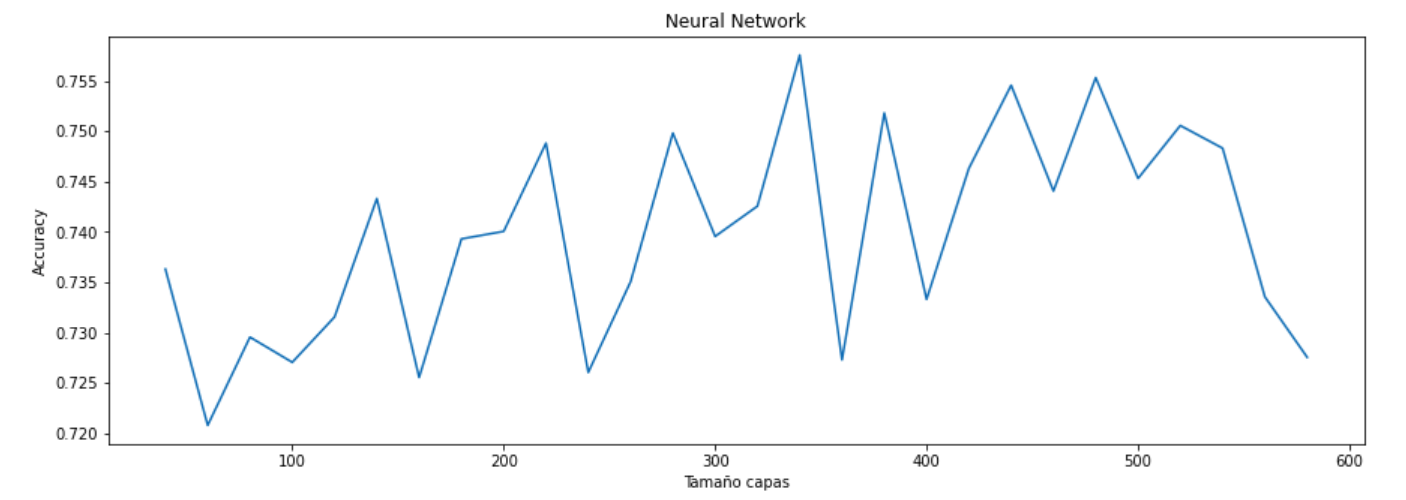
\includegraphics[width=0.9\linewidth]{img/nn1}
	\caption{}
	\label{fig:nn1}
\end{figure}

y el tamaño de capas para el que la precisión es mayor es entonces 340: 
\begin{minted}{python}
NN=MLPClassifier(hidden_layer_sizes=(340,340),random_state=10,max_iter=1000)
cross_validation(NN, df_train_norm, df_train_obj,True)

Accuracy:  0.7575505617977528
\end{minted}

Llevamos ahora a cabo un Grid Search, en el que especificamos algunos tamaños aleatorios para tres capas y las dos capas con el mejor tamaño que acabamos de encontrar (para ver si con tres capas los resultados son mejores), y algunos valores para el parámetro de regularización alpha (cuanto mayor sea este parámetro más influencia tendrá la regularización, reduciéndose así el overfitting):
\begin{minted}{python}
from sklearn.model_selection import GridSearchCV

mlp=MLPClassifier(random_state=10)
parameter_space = {
'hidden_layer_sizes': [(200,100,100),(300,200,100),(200,100,50),(340,340)],
'alpha': [0.001, 0.0003,0.0015,0.01,0.02,0.1,],
'max_iter':[10000],
}

clf=GridSearchCV(mlp, parameter_space, n_jobs=-1, cv=5)
clf.fit(df_train_norm, df_train_obj)

print('Mejores parámetros: ', clf.best_params_)

Mejores parámetros:  {'alpha': 0.0015, 'hidden_layer_sizes': (300, 200, 100), 
'max_iter': 10000}
\end{minted}

Comprobamos que efectivamente con tres capas de tamaños (300,200,100) el resultado mejora un poco:
\begin{minted}{python}
NN=MLPClassifier(hidden_layer_sizes=(300,200,100),random_state=10,max_iter=1000,
alpha=0.0015)
cross_validation(NN,df_train_norm,df_train_obj,True)

Accuracy:  0.7578021223470662
\end{minted}

Así pues, nos quedamos con estos valores de los parámetros, y usamos estas redes neuronales para clasificar el conjunto de test.\newpage 
\subsection{Características de la entrega}
\begin{table}[htbp]
	\caption{}\begin{center}
		\begin{tabular}{|c|c|c|c|c|}
			\hline
			\multicolumn{1}{|l|}{\textbf{}} & \textbf{} & \textbf{} & \multicolumn{ 2}{c|}{\textbf{Score}} \\ \hline
			\textbf{Entrega} & \textbf{Fecha y Hora} & \textbf{Posición en Ranking (hasta ese momento)} & \textbf{Train} & \textbf{Test} \\ \hline
			\textbf{1} & 23 de diciembre 21:30 & 10 & 0.822526 & 0.74374 \\ \hline
			\textbf{2} &  24 de diciembre  16:51 & 10 & 0.8245411 & 0.74029 \\ \hline
			\textbf{3} & 24  de diciembre 19:49 & 13 & 0.8102943 & 0.72389 \\ \hline
			\textbf{4} & 24 de diciembre 21:00  & 7 & 0.836037 & 0.76704 \\ \hline
			\textbf{5} &  25 de diciembre 13:07 & 7 & 0.8147927 & 0.73856 \\ \hline
			\textbf{6} & 25  de diciembre  19:10  & 7 & 0.757802 & 0.69801 \\ \hline
	\end{tabular}\end{center}
	\label{}
\end{table}

Así, el resultado para las redes neuronales es el peor obtenido hasta el momento. Esto puede ser debido a que las redes neuronales necesitan de una configuración de parámetros muy exhaustiva, lo cual no hemos llegado a hacer aquí, por lo que con una mejor configuración habría sido posible que los resultados mejoraran. 

\section{Entrega 7}
\subsection{Preprocesamiento}
Seguimos con el preprocesamiento usado en todas las entregas anteriores
\subsection{Aplicación de los algoritmos}
Una vez que ya tenemos los mejores modelos con sus parámetros configurados, vamos a hacer un \textbf{Stacking} de todos ellos usando el \mintinline{python}{StackingClassifier} de sklearn. Este se encarga de apilar la salida de varios estimadores individuales y usa un clasificador último que recibe como entrada las salidas de cada uno de ellos y calcula la predicción final, de manera que se aúnan las fortalezas de cada uno de los estimadores y sus debilidades se ven reducidas, obteniendo en la mayoría de los casos un resultado igual de bueno que el proporcionado por el mejor de los estimadores o incluso mejor. 

Así pues, consideramos nuestra Red Neuronal, Gradient Boosting, clasificador de Extra-Trees, Random Forest y Bagging de Knn, y probamos a hacer stacking de todos ellos:
\begin{minted}{python}
estimators = [('red neuronal',NN),('bagging_knn', bagging_knn),
('forest', forest),('extra_trees', extra),('gradient',gradient)]

clf = StackingClassifier(estimators=estimators, final_estimator=forest,cv=5)
cross_validation(clf, df_train_norm, df_train_obj,True)

Accuracy:  0.8350374531835205
\end{minted}

solo con algunos:
\begin{minted}{python}
estimators = [('forest', forest),('extra_trees', extra),('gradient',gradient)]

clf = StackingClassifier(estimators=estimators, final_estimator=forest,cv=5)
cross_validation(clf, df_train_norm, df_train_obj,True)

Accuracy:  0.8317887016229714
\end{minted}
variando el clasificador final:

\begin{minted}{python}
estimators = [('red neuronal',NN),('bagging_knn', bagging_knn),('forest', forest),
('extra_trees', extra),('gradient',gradient)]

clf = StackingClassifier(estimators=estimators, final_estimator=NN,cv=5)
cross_validation(clf, df_train_norm, df_train_obj,True)

Accuracy:  0.8295455680399499
\end{minted}

e incluso intentamos varias capas de Stacking:
 
 \begin{minted}{python}
capa1_estimadores=[('forest', forest),('extra_trees', extra),
('gradient',gradient),('bagging_knn', bagging_knn)]
capa2_estimadores=[('forest', forest),('gradient',gradient)]
capa2=StackingClassifier(estimators=capa2_estimadores, final_estimator=forest,cv=5)
clf = StackingClassifier(estimators=capa1_estimadores, final_estimator=capa2,cv=5)
cross_validation(clf, df_train_norm, df_train_obj,True)

Accuracy:  0.8197946317103622
 \end{minted}

para ver qué opción nos da los mejores resultados (he probado otras opciones para los estimadores que no he recogido en la memoria, pero se pueden ver en el notebook \mintinline{python}{p3_6.ipynb}).

De todas las pruebas realizadas, la que nos proporciona un valor de accuracy más alto es la primera que hemos incluido aquí, es decir, en la que consideramos todos los clasificadores y tomamos Random Forest como clasificador final. Por lo tanto, entrenamos el StackingClassifier con dichos estimadores con el conjunto de entrenamiento preprocesado en el que eliminamos todos los nulos (pues este era el preprocesamiento que mejores resultados daba en la mayoría de los estimadores que hemos incluido en el stacking, de ahí que nos hayamos centrado en este en todas las entregas anteriores) y lo usamos para predecir las clases del conjunto de test.\newpage

\subsection{Características de la entrega}
\begin{table}[htbp]
	\caption{}\begin{center}
	\begin{tabular}{|c|c|c|c|c|}
		\hline
		\multicolumn{1}{|l|}{\textbf{}} & \textbf{} & \textbf{} & \multicolumn{ 2}{c|}{\textbf{Score}} \\ \hline
		\textbf{Entrega} & \textbf{Fecha y Hora} & \textbf{Posición en Ranking (hasta ese momento)} & \textbf{Train} & \textbf{Test} \\ \hline
		\textbf{1} & 23 de diciembre 21:30 & 10 & 0.822526 & 0.74374 \\ \hline
		\textbf{2} &  24 de diciembre  16:51 & 10 & 0.8245411 & 0.74029 \\ \hline
		\textbf{3} & 24  de diciembre 19:49 & 13 & 0.8102943 & 0.72389 \\ \hline
		\textbf{4} & 24 de diciembre 21:00  & 7 & 0.836037 & 0.76704 \\ \hline
		\textbf{5} &  25 de diciembre 13:07 & 7 & 0.8147927 & 0.73856 \\ \hline
		\textbf{6} & 25  de diciembre  19:10  & 7 & 0.757802 & 0.69801 \\ \hline
		\textbf{7} & 25 de diciembre 19:24 & 7 & 0.835037 & 0.77308 \\ \hline
	\end{tabular}\end{center}
	\label{}
\end{table}

Al hacer el stacking de los clasificadores, los resultados han mejorado con respecto a los proporcionados por uno solo de ellos, como era de esperar. 

\section{Entrega 8}
\subsection{Preprocesamiento}
Vamos a probar ahora a realizar un preprocesamiento diferente. En concreto, en lugar de transformar las variables categóricas a numéricas usando LabelEncoder, vamos a convertirlas a binario usando One-Hot Encoding. Además, el conjunto de entrenamiento presenta un notable desbalanceo de clases:
\begin{minted}{python}
Counter(df_train_obj)

Counter({3: 1825, 2: 502, 4: 834, 5: 637, 1: 203})
\end{minted}

La clase mayoritaria cuenta con 1825 instancias mientras que la minoritaria cuenta solo con 203.  Por lo tanto, vamos a intentar reducir este desbalanceo usando técnicas de oversampling y undersampling. 

Así pues, comenzamos preprocesando tanto el conjunto de entrenamiento como el de test eliminando las columnas de id y descuento y tratando los valores nulos como hemos hecho hasta ahora (para un caso eliminamos todas las instancias nulas y para otro sustituimos las instancias nulas de asientos por el valor más frecuente y eliminamos el resto de nulos, obteniendo así dos conjuntos de datos de entrenamiento diferentes, que nombramos como ya comentamos al principio \mintinline{python}{df_train} y \mintinline{python}{df_train_replaced} respectivamente). Después separamos ambos conjuntos de datos en atributos a usar para el entrenamiento y clases objetivo a predecir. Normalizamos seguidamente solo las variables numéricas, usando MinMaxScaler de la misma forma que ya explicamos para la primera entrega. 

A continuación, aplicamos el One-Hot Enconder de sklearn de la siguiente forma:

\begin{minted}{python}
categorical=["nombre","ciudad","combustible","tipo_marchas",
"mano","consumo","motor_cc","potencia"]
cols = [col for col in df_train.columns if col not in categorical]    

df_train_num=df_train_norm.copy()
df_train_num_rpl=df_train_norm_rpl.copy()
df_test_num=df_test_norm.copy()

df_train_num=np.array(df_train_num[cols])
df_train_num_rpl=np.array(df_train_num_rpl[cols])
df_test_num=np.array(df_test_num[cols])

for atributo in categorical:
	data=pd.read_csv("data/"+atributo+".csv")
	data.columns = [col.lower() for col in data]
	enc = OneHotEncoder().fit(data[atributo].values.reshape(-1,1))
	
	#Conjunto de entrenamiento con ambos preprocesamientos
	enc_train=enc.transform(df_train[atributo].values.reshape(-1,1)).toarray()        
	df_train_num=np.hstack((df_train_num,enc_train))
	
	enc_train_rpl=
	enc.transform(df_train_replaced[atributo].values.reshape(-1,1)).toarray()
	
	df_train_num_rpl=np.hstack((df_train_num_rpl,enc_train_rpl))
	
	
	#Conjunto de test
	enc_test=enc.transform(df_test[atributo].values.reshape(-1,1)).toarray()
	df_test_num=np.hstack((df_test_num,enc_test))

df_train_num=pd.DataFrame(df_train_num)
df_train_num_rpl=pd.DataFrame(df_train_num_rpl)
df_test_num=pd.DataFrame(df_test_num)
\end{minted}

En primer lugar hemos hecho una copia de los conjuntos de datos normalizados procedentes de la fase de preprocesamiento anterior, con los que vamos a trabajar. Nos quedamos sólo con los atributos numéricos de los mismos y convertimos los DataFrames a arrays de Numpy. Después aplicamos el OneHotEncoder a cada uno de los DataFrames correspondientes a los archivos 'atributo.csv' que contienen los valores de las variables categóricas y transformamos entonces a binario, usando las correspondencias aprendidas, los atributos correspondientes en ambos conjuntos de entrenamiento y en el conjunto de test, pasando los resultados a arrays. Unimos a continuación el array resultante de la conversión del atributo en cada caso a los conjuntos iniciales formados solo por las variables numéricas. Finalmente, volvemos a convertir los conjuntos a DataFrames de pandas y vemos el resultado:

\begin{figure}[H]
	\centering
	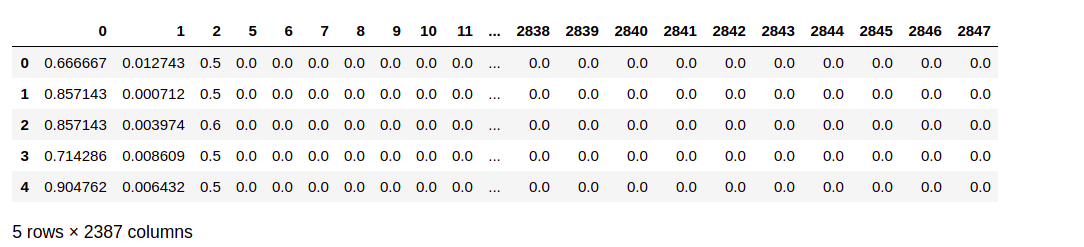
\includegraphics[width=1\linewidth]{img/onehot1}
	\caption{}
	\label{fig:onehot1}
\end{figure}


Así, para cada atributo categórico han aparecido varias columnas de 0's y 1's que recogen los valores que toma el mismo. 

\begin{figure}[H]
	\centering
	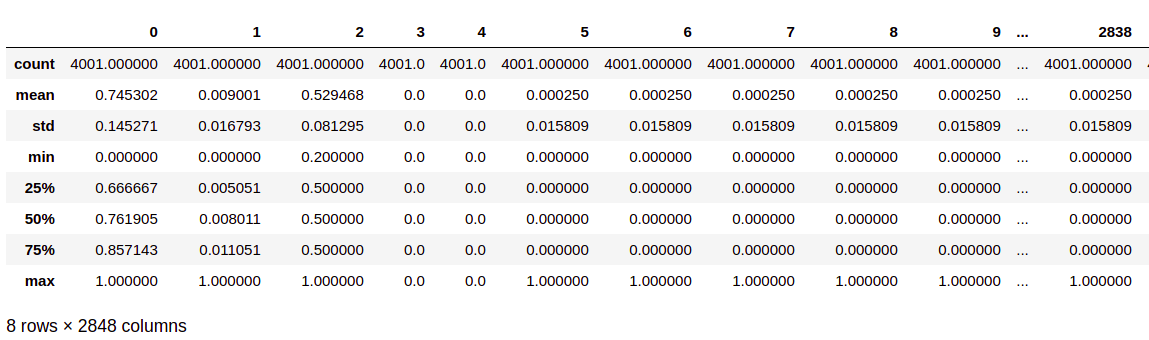
\includegraphics[width=1\linewidth]{img/onehot2}
	\caption{}
	\label{fig:onehot2}
\end{figure}

Como aparecen columnas que son todo nulas, y no aportan por lo tanto información, las eliminamos. Para ello, buscamos las que tienen como valor máximo un 0 y no las consideramos:
\begin{minted}{python}
cols = [col for col in df_train_num.columns if df_train_num[col].max()!=0.0]
df_train_num=df_train_num[cols]
df_test_num=df_test_num[cols]
df_train_num_rpl=df_train_num_rpl[cols]
\end{minted}

Pasamos entonces ahora a aplicar los algoritmos de \textbf{oversampling} y \textbf{undersampling}.

Por una parte, para llevar a cabo el oversampling vamos a usar el algoritmo de SMOTE de \mintinline{python}{imblearn}, usando como \mintinline{python}{sampling_strategy} el valor por defecto, esto es, creando más muestras de todas las clases menos de la mayoritaria. Aplicamos entonces dicho algoritmo a los dos conjuntos de entrenamiento con los diferentes preprocesamientos que venimos considerando: 
\begin{minted}{python}
smote=SMOTE(random_state=10)
df_train_over, df_train_obj_over = smote.fit_resample(df_train_num, df_train_obj)
df_train_over_rpl, df_train_obj_over_rpl = 
smote.fit_resample(df_train_num_rpl, df_train_obj_replaced)

Counter(df_train_obj_over)

Counter({3: 1825, 2: 1825, 4: 1825, 5: 1825, 1: 1825})
\end{minted}

y observamos que ahora cada clase posee el mismo número de instancias, que de hecho es la cantidad de instancias que tenía la clase mayoritaria. 

Por otra parte, para el undersampling usamos EditedNearestNeighbours también de \mintinline{python}{imblearn}, con \mintinline{python}{sampling_strategy} por defecto, es decir, eliminando instancias de todas las clases menos de la minoritaria, y considerando 5 vecinos:
\begin{minted}{python}
resampler=EditedNearestNeighbours(n_neighbors=5)
df_train_under, df_train_obj_under = resampler.fit_resample(df_train_num, df_train_obj)
df_train_under_rpl, df_train_obj_under_rpl =
 resampler.fit_resample(df_train_num_rpl, df_train_obj_replaced)

Counter(df_train_obj_under)

Counter({1: 203, 2: 31, 3: 812, 4: 256, 5: 408})
\end{minted}

y vemos que ahora el número de instancias de cada clase se ha reducido, menos las de la clase minoritaria que era la 1. En este caso sigue habiendo desbalanceo de clases, aunque ahora no es tan notable como el original. 

\subsection{Aplicación de los algoritmos}

Tras aplicar los algoritmos que venimos considerando hasta ahora con parámetros por defecto a los datos de entrenamiento con estos nuevos preprocesamientos, los valores de accuracy obtenidos usando la función \mintinline{python}{cross_validation} han sido los siguientes:

\begin{table}[htbp]
	\caption{}\begin{center}
	\begin{tabular}{|c|r|r|l|r|}
		\hline
		\multicolumn{1}{|l|}{} & \multicolumn{ 4}{c|}{\textbf{Nulos reemplazados en asientos}} \\ \hline
		\multicolumn{1}{|l|}{} & \multicolumn{1}{l|}{\textit{Clases desbalanceadas}} & \multicolumn{1}{l|}{\textit{Oversampling}} & \textit{} & \multicolumn{1}{l|}{\textit{Undersampling}} \\ \hline
		LinearSVC & 0.752774 & 0.88534 &  & 0.9539 \\ \hline
		Knn & 0.747598 & 0.8654 &  & 0.94208 \\ \hline
		RandomForest & 0.787528 & 0.93663 &  & 0.95271 \\ \hline
		DecisionTree & 0.74784 & 0.88997 &  & 0.93734 \\ \hline
		Red Neuronal & 0.756223 & 0.93857 &  & 0.94799 \\ \hline
		Extra-Trees & 0.776929 & 0.94288 &  & 0.95507 \\ \hline
		Gradient Boosting & 0.756717 & 0.85344 &  & 0.94442 \\ \hline
	\end{tabular}\end{center}
	\label{}
\end{table}

\begin{table}[htbp]
	\caption{}\begin{center}
		\begin{tabular}{|c|r|r|l|r|}
			\hline
			\multicolumn{1}{|l|}{} & \multicolumn{ 4}{c|}{\textbf{Nulos eliminados}} \\ \hline
			\multicolumn{1}{|l|}{} & \multicolumn{1}{l|}{\textit{Clases desbalanceadas}} & \multicolumn{1}{l|}{\textit{Oversampling}} & \textit{} & \multicolumn{1}{l|}{\textit{Undersampling}} \\ \hline
				LinearSVC & 0.752811 & 0.889753 & & 0.956725 \\ \hline
			Knn & 0.748813 & 0.864328 & & 0.943274 \\ \hline
			RandomForest & 0.792301 & 0.936219 & & 0.957309 \\ \hline
			DecisionTree & 0.743313 & 0.888328 & & 0.935087 \\ \hline
			Red Neuronal & 0.755061 & 0.937863 & & 0.952046 \\ \hline
			Extra-Trees & 0.774558 & 0.941479 & & 0.957309 \\ \hline
			Gradient Boosting & 0.767806 & 0.859835 & & 0.94269 \\ \hline
	\end{tabular}\end{center}
	\label{}
\end{table}

Nos damos cuenta de que el \textbf{undersampling} nos da los mejores valores de accuracy, de manera que por ahora vamos a centrarnos en este preprocesamiento. Además, con todos los nulos eliminados, incluidos los de la columna de asientos, obtenemos mejores resultados para casi todos los algoritmos, y en los que estos son inferiores la diferencia es mínima, con lo que nos vamos a quedar también con este conjunto de datos. 

\subsection{Configuración de parámetros}

Nos centramos en esta entrega en las máquinas de soporte vectorial lineales y configuramos el parámetro de regularización C. Para ello usamos la siguiente función:
\begin{minted}{python}
def tune_svc(max_value,data,obj):
	acc=[]
	for i in range(1,max_value):
		svc=LinearSVC(random_state=10,C=i,max_iter=100000)
		acc.append(cross_validation(svc,data,obj))
	
	fig, ax =plt.subplots(figsize=(15,5))
	ax.plot(range(1,max_value), acc)
	ax.set_title('Linear SVC')
	ax.set_xlabel('Valor parámetro')
	ax.set_ylabel('Accuracy')
	plt.show()
\end{minted}

que itera sobre un rango de valores del parámetro C considerado, almacena los resultados de la precisión de cada iteración y finalmente los muestra gráficamente. Si ejecutamos la función con un valor máximo de 15 y con los datos de entrenamiento resultantes del preprocesado con undersampling, la salida es la siguiente: 

\begin{figure}[H]
	\centering
	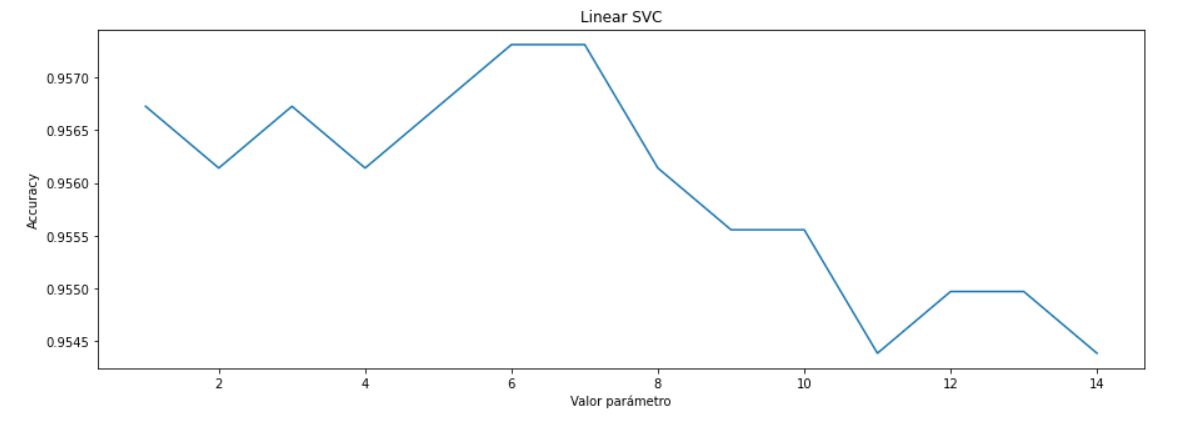
\includegraphics[width=0.9\linewidth]{img/svc1}
	\caption{}
	\label{fig:svc1}
\end{figure}

donde podemos observar que los mejores restultados se obtienen para un valor del parámetro de 6. 

Por lo tanto, entrenamos el LinearSVC con $C=6$ sobre el conjunto de entrenamiento completo preprocesado como ya hemos comentado y con undersampling y lo usamos para predecir las clases del conjunto de test:

\begin{minted}{python}
svc=LinearSVC(random_state=10,C=6,max_iter=100000)
cross_validation(svc, df_train_under,df_train_obj_under,True)
svc.fit(df_train_under,df_train_obj_under)
pred=svc.predict(df_test_num)
ids=df_test_orig["id"]

df_result = pd.DataFrame({'id': ids, 'Precio_cat': pred})
df_result.to_csv("resultados_8.csv", index=False)
\end{minted}
\newpage
\subsection{Características de la entrega}
\begin{table}[htbp]
	\caption{}\begin{center}
	\begin{tabular}{|c|c|c|c|c|}
		\hline
		\multicolumn{1}{|l|}{\textbf{}} & \textbf{} & \textbf{} & \multicolumn{ 2}{c|}{\textbf{Score}} \\ \hline
		\textbf{Entrega} & \textbf{Fecha y Hora} & \textbf{Posición en Ranking (hasta ese momento)} & \textbf{Train} & \textbf{Test} \\ \hline
		\textbf{8} & 26 de diciembre 20:04 & 9 & \multicolumn{1}{r|}{0.957309} & 0.61087 \\ \hline
	\end{tabular}\end{center}
	\label{}
\end{table}

Y nos damos cuenta de que los resultados en Kaggle son bastante pobres.

\section{Entrega 9}

Para esta entrega partimos de los datos preprocesados como en la entrega anterior y simplemente vamos a entrenar un Random Forest con parámetros por defecto sobre el conjunto de entrenamiento. A continuación usamos dicho clasificador para predecir las clases del conjunto de test y subimos los resultados a Kaggle para ver cómo se comporta Random Forest con este preprocesamiento:

\begin{minted}{python}
forest=RandomForestClassifier(random_state=10)
cross_validation(forest, df_train_under,df_train_obj_under,True)
forest.fit(df_train_under,df_train_obj_under)
pred=forest.predict(df_test_num)
ids=df_test_orig["id"]

df_result = pd.DataFrame({'id': ids, 'Precio_cat': pred})
df_result.to_csv("resultados_9.csv", index=False)
\end{minted}

\subsection{Características de la entrega}
\begin{table}[htbp]
	\caption{}\begin{center}
	\begin{tabular}{|c|c|c|c|c|}
		\hline
		\multicolumn{1}{|l|}{\textbf{}} & \textbf{} & \textbf{} & \multicolumn{2}{c|}{\textbf{Score}} \\ \hline
		\textbf{Entrega} & \textbf{Fecha y Hora} & \textbf{Posición en Ranking (hasta ese momento)} & \textbf{Train} & \textbf{Test} \\ \hline
		\textbf{8} & 26 de diciembre 20:04 & 9 & 0.957309 & 0.61087 \\ \hline
		\textbf{9} & 26 de diciembre 20:06 & 9 & 0.957309 & 0.61259 \\ \hline
	\end{tabular}\end{center}
	\label{}
\end{table}

Los resultados son bastante bajos nuevamente, aunque algo mejores que con LinearSVC.
\section{Entrega 10}
\subsection{Preprocesamiento}
Para esta entrega seguimos con el mismo preprocesamiento que el realizado en las dos entregas anteriores: eliminación de todos los nulos, normalización de datos numéricos,  transformación de variables categóricas a binario usando One-Hot Enconding y Undersampling con EditedNearestNeighbours para lidiar con el desbalanceo de clases. 
\subsection{Configuración de parámetros}
Estudiamos ahora qué número de vecinos es más adecuado para nuestros datos en el algoritmo de los vecinos más cercanos usando la siguiente función:
\begin{minted}{python}
def tune_knn(max_value,data,obj):
	acc=[]
	for i in range(2,max_value):
		knn=KNeighborsClassifier(n_neighbors=i)
		acc.append(cross_validation(knn,data,obj))
	
	fig, ax =plt.subplots(figsize=(15,5))
	ax.plot(range(2,max_value), acc)
	ax.set_title('vecino más cercano')
	ax.set_xlabel('Num vecinos')
	ax.set_ylabel('Accuracy')
	plt.show()

\end{minted}
cuyo funcionamiento es igual al del resto de funciones que venimos usando para tunear los parámetros. Ejecutando \mint{python}{tune_knn(20,df_train_under,df_train_obj_under)} obtenemos:
\begin{figure}[H]
	\centering
	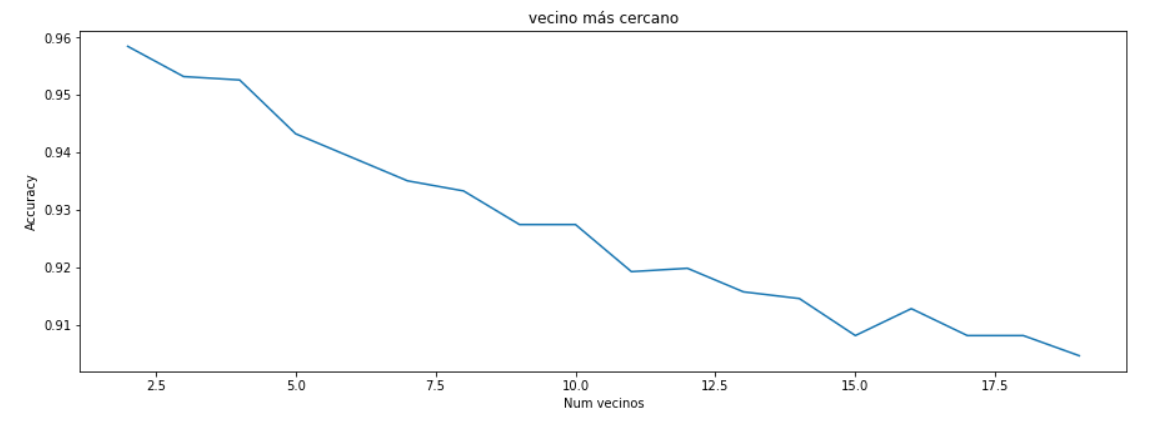
\includegraphics[width=0.9\linewidth]{img/knn3}
	\caption{}
	\label{fig:knn3}
\end{figure}


de manera que con dos vecinos los resultados son los mejores. 

\subsection{Aplicación de los algoritmos}

Intentamos ahora mejorar los resultados obtenidos en Kaggle para este preprocesamiento probando a hacer Stacking de algunos de los clasificadores, la mayoría con parámetros por defecto, salvo en el caso de LinearSVC y Knn, en los que hemos considerado los mejores valores de los parámetros configurados. 

De las opciones probadas, la que presenta un valor más alto de la precisión es la siguiente:
\begin{minted}{python}
extra=ExtraTreesClassifier(random_state=10)
svc=LinearSVC(random_state=10,C=6,max_iter=100000)
knn=KNeighborsClassifier(n_neighbors=2)
forest=RandomForestClassifier(random_state=10)
NN=MLPClassifier(random_state=10,max_iter=10000)

estimators = [('Linear SVC', svc),
('forest', forest),('extra_trees', extra),('Red Neuronal',NN),('knn',knn)]

clf = StackingClassifier(estimators=estimators, final_estimator=forest,cv=5)
cross_validation(clf, df_train_under, df_train_obj_under,True)
\end{minted}

que nos da \mintinline{python}{Accuracy:  0.9719298245614034}, por lo que vamos a usar el clasificador resultante de este Stacking para clasificar el conjunto de test y subir los resultados a Kaggle.

\subsection{Características de la entrega}

\begin{table}[htbp]
	\caption{}\begin{center}
	\begin{tabular}{|c|c|c|c|c|}
		\hline
		\multicolumn{1}{|l|}{\textbf{}} & \textbf{} & \textbf{} & \multicolumn{ 2}{c|}{\textbf{Score}} \\ \hline
		\textbf{Entrega} & \textbf{Fecha y Hora} & \textbf{Posición en Ranking (hasta ese momento)} & \textbf{Train} & \textbf{Test} \\ \hline
		\textbf{8} & 26 de diciembre 20:04 & 9 & 0.957309 & 0.61087 \\ \hline
		\textbf{9} & 26 de diciembre 20:06 & 9 & 0.957309 & 0.61259 \\ \hline
		\textbf{10} & 26 de diciembre 23:03 & 9 & 0.971929 & 0.62295 \\ \hline
	\end{tabular}\end{center}
	\label{}
\end{table}


Así, el resultado ha mejorado un poco pero sigue siendo muy bajo comparado con los obtenidos en las primeras entregas.

\textbf{Nota:} No sé por qué seguí intentando mejorar los resultados y haciendo entregas con este preprocesamiento, si desde la primera entrega que hice con él ya se veía que solo empeoraba los resultados. Por eso no configuré el resto de clasificadores usados en el stacking, estaba viendo que este preprocesamiento no llevaba a ningún lado. 

De hecho, es lógico que los resultados sean tan bajos, puesto que los clasificadores se están entrenando con muchas menos instancias. Además, las datos pertenecientes a la clase 2 que aparezcan en el test, es muy probable que no se clasifiquen correctamente, pues, como pudimos comprobar en las clases resultantes tras aplicar el undersampling, en el conjunto de entrenamiento quedaron sólo 31 instancias de la clase 2.
\section{Entrega 11}
\subsection{Preprocesamiento}
Teniendo ya pruebas suficientes de que el undersampling no da buenos resultados, vamos a estudiar lo que ocurre haciendo oversampling con el algoritmo de Smote sobre el conjunto de entrenamiento. 
Así pues, partimos de los datos preprocesados como hasta ahora, con la única diferencia de que esta vez usaremos la técnica de Oversampling en lugar de Undersampling para deshacernos del problema del desbalanceo de las clases. 

\subsection{Aplicación de los algoritmos}
En este caso, en vez de empezar configurando los parámetros de los mejores algoritmos, como hicimos en otras entregas, vamos a usar los parámetros que los mismos traen por defecto y vamos a apilar algunos de los algoritmos con un Stacking, para analizar los resultados y ver cuán útil es la técnica de oversampling.

Tras probar varias opciones para los estimadores usados en el stacking y para el estimador final, la siguiente ha resultado ser mejor:
\begin{minted}{python}
extra=ExtraTreesClassifier(random_state=10)
svc=LinearSVC(random_state=10)
forest=RandomForestClassifier(random_state=10)
NN=MLPClassifier(random_state=10,max_iter=10000)


estimators = [('Linear SVC', svc),
('forest', forest),('extra_trees', extra),('Red Neuronal',NN)]

clf = StackingClassifier(estimators=estimators, final_estimator=forest,cv=5,n_jobs=6)
cross_validation(clf, df_train_over, df_train_obj_over,True)
\end{minted}

que nos ofrece \mintinline{python}{Accuracy:  0.9507945205479453}. Usamos pues el clasificador resultante de este Stacking para predecir las clases de los datos del conjunto de test y entregamos las predicciones. 

\subsection{Características de la entrega}

\begin{table}[htbp]
	\caption{}
	\begin{tabular}{|c|c|c|c|c|}
		\hline
		\multicolumn{1}{|l|}{\textbf{}} & \textbf{} & \textbf{} & \multicolumn{ 2}{c|}{\textbf{Score}} \\ \hline
		\textbf{Entrega} & \textbf{Fecha y Hora} & \textbf{Posición en Ranking (hasta ese momento)} & \textbf{Train} & \textbf{Test} \\ \hline
		\textbf{10} & 26 de diciembre 23:03 & 9 & 0.971929 & 0.62295 \\ \hline
		\textbf{11} & 27 de diciembre  17:43 & 9 & 0.95079 & 0.71786 \\ \hline
	\end{tabular}
	\label{}
\end{table}

El resultado es algo más prometedor en este caso, aunque sigue siendo bajo. Esto puede ser debido a que hemos incluido en el stacking modelos que ofrecen peores resultados, lo que hace que en conjunto los resultados sean peores. Además, no hemos configurado ninguno de sus parámetros, lo cual es otro motivo para que baje el resultado. 

\section{Entrega 12}
\subsection{Preprocesamiento}

Seguimos con el mismo preprocesamiento que usamos para la entrega anterior: eliminación de todos los nulos, normalización de datos numéricos, transformación de variables categóricas a binario usando One-Hot Enconding y Oversampling con el algoritmo de SMOTE para eliminar el problema del desbalanceo de clases.

\subsection{Configuración de parámetros}

Como vimos en el Cuadro 11, donde comparábamos los resultados de varios algoritmos para los distintos preprocesamientos, el clasificador de Extra-Trees presenta el valor más alto de la precisión para el preprocesamiento que aquí hemos considerado. Por lo tanto, vamos a centrarnos en configurar los parámetros del mismo.  

En primer lugar comprobamos si activar la opción de bootstrap mejora los resultados, pero no lo hace, así que dejamos su valor a False. A continuación buscamos el número de árboles más apropiado usando la función:
\begin{minted}{python}
def tune_num_arboles(max_value):
	acc=[]
	for i in range(5,max_value,20):
		extra=ExtraTreesClassifier(n_estimators=i,random_state=10)
		acc.append(cross_validation(extra,df_train_over,df_train_obj_over))
	
	fig, ax =plt.subplots(figsize=(15,5))
	ax.plot(range(5,max_value,20), acc)
	ax.set_title('Extra trees')
	ax.set_xlabel('Num árboles')
	ax.set_ylabel('Accuracy')
	plt.show()
\end{minted} 

que aplicada para un \mintinline{python}{max_value=300} nos muestra:
\begin{figure}[H]
	\centering
	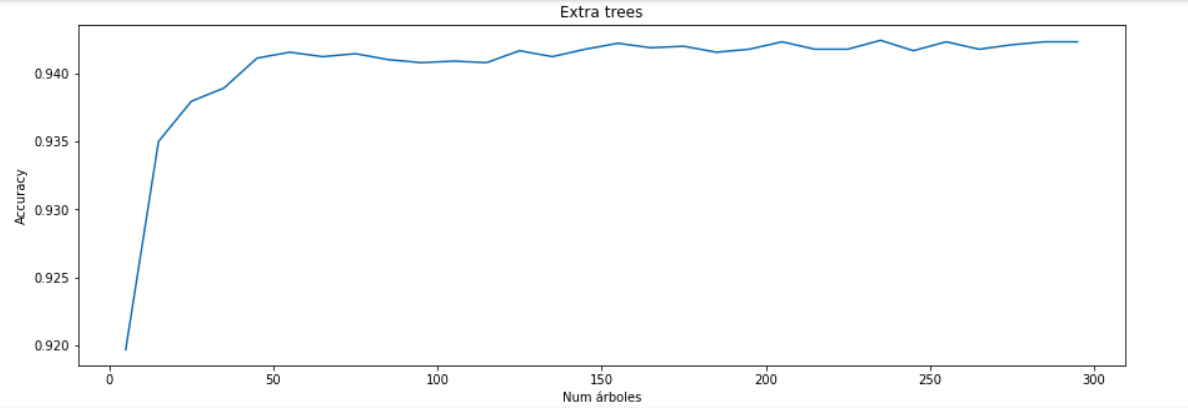
\includegraphics[width=0.9\linewidth]{img/extra3}
	\caption{}
	\label{fig:extra3}
\end{figure}

y entonces el mejor valor de accuracy se obtiene para \mintinline{python}{n_estimators=275}:

\begin{minted}{python}
extra=ExtraTreesClassifier(n_estimators=275,random_state=10)
cross_validation(extra, df_train_over, df_train_obj_over,True)

Accuracy:  0.94213698630137
\end{minted}

Finalmente estudiamos si se produce alguna mejora al cambiar el parámetro \mintinline{python}{max_depht}. Pero al probar algunos valores aleatorios del mismo, observamos que los resultados empeoran en todos los casos, por lo que lo dejamos también con su valor por defecto, que  es sin restricciones de profundidad en cada árbol.

Una vez que ya sabemos los valores más adecuados para algunos de los parámetros del clasificador considerado, procedemos a entrenarlo con dichos valores de los parámetros con el conjunto de entrenamiento preprocesado como ya hemos comentado y a predecir con él las clases de las instancias del conjunto de test:

\begin{minted}{python}
extra=ExtraTreesClassifier(n_estimators=275,random_state=10)
cross_validation(extra, df_train_over, df_train_obj_over,True)
extra.fit(df_train_over,df_train_obj_over)
pred=extra.predict(df_test_num)
ids=df_test_orig["id"]

df_result = pd.DataFrame({'id': ids, 'Precio_cat': pred})
df_result.to_csv("resultados_12.csv", index=False)
\end{minted}

\subsection{Características de la entrega}
\begin{table}[htbp]
	\caption{}
	\begin{tabular}{|c|c|c|c|c|}
		\hline
		\multicolumn{1}{|l|}{\textbf{}} & \textbf{} & \textbf{} & \multicolumn{ 2}{c|}{\textbf{Score}} \\ \hline
		\textbf{Entrega} & \textbf{Fecha y Hora} & \textbf{Posición en Ranking (hasta ese momento)} & \textbf{Train} & \textbf{Test} \\ \hline
		\textbf{11} & 27 de diciembre  17:43 & 9 & 0.9524383 & 0.71786 \\ \hline
		\textbf{12} & 27 de diciembre 18:23 & 9 & 0.942136 & 0.70578 \\ \hline
	\end{tabular}
	\label{}
\end{table}

Podemos observamos que el resultado no es muy bueno.

\section{Entrega 13}
\subsection{Preprocesamiento}

Viendo que no obtenemos buenos resultados con el preprocesamiento anterior, vamos a modificar éste ligeramente. Como en la técnica de oversampling se crean instancias nuevas, puede ocurrir que se esté introduciendo ruido en el conjunto de entrenamiento y los algoritmos se dejen llevar por dicho ruido, lo que hace que empeoren los resultados sobre el conjunto de test. Para intentar reducir este efecto, en lugar de considerar como \mintinline{python}{sampling_strategy} en el algoritmo de SMOTE la opción por defecto, vamos a probar con 'minority', de manera que sólo se crean más instancias de la clase minoritaria, y las instancias de las demás clases no se ven modificadas. 

Así, llevamos a cabo el preprocesamiento como en las últimas entregas y en el algoritmo de SMOTE establecemos \mintinline{python}{sampling_strategy='minority'}. 

Cabe mencionar también que vamos a trabajar con los datos en que eliminamos todas las instancias nulas.

\subsection{Aplicación de los algoritmo}

Para tener una primera idea de cómo de buena es esta solución, vamos a hacer un stacking de algunos algoritmos con sus parámetros por defecto, como hicimos para la entrega 11.

De todas las opciones probadas, la que ofrece los mejores resultados es la siguiente:
\begin{minted}{python}
extra=ExtraTreesClassifier(random_state=10)
gradient=GradientBoostingClassifier(random_state=10,max_features='auto')
svc=LinearSVC(random_state=10)
tree=DecisionTreeClassifier(random_state=10)
forest=RandomForestClassifier(random_state=10)
NN=MLPClassifier(random_state=10,max_iter=10000)


estimators = [('Linear SVC', svc),('gradient',gradient),
('forest', forest),('extra_trees', extra),('Red Neuronal',NN),('decision tree',tree)]

clf = StackingClassifier(estimators=estimators, final_estimator=forest,cv=5,n_jobs=6)
cross_validation(clf, df_train_over, df_train_obj_over,True) 

Accuracy:  0.8788909450375643
\end{minted}

con lo que la usamos para clasificar los datos del conjunto de test y subir los resultados a Kaggle.

\subsection{Características de la entrega}

\begin{table}[htbp]
	\caption{}\begin{center}
	\begin{tabular}{|c|c|c|c|c|}
		\hline
		\multicolumn{1}{|l|}{\textbf{}} & \textbf{} & \textbf{} & \multicolumn{ 2}{c|}{\textbf{Score}} \\ \hline
		\textbf{Entrega} & \textbf{Fecha y Hora} & \textbf{Posición en Ranking (hasta ese momento)} & \textbf{Train} & \textbf{Test} \\ \hline
		\textbf{11} & 27 de diciembre  17:43 & 9 & 0.9524383 & 0.71786 \\ \hline
		\textbf{12} & 27 de diciembre 18:23 & 9 & 0.942136 & 0.70578 \\ \hline
		\textbf{13} & 27 de diciembre 21:49 & 10 & 0.87889 & 0.73166 \\ \hline
	\end{tabular}\end{center}
	\label{}
\end{table}

Vemos que efectivamente los resultados han mejorado un poco con respecto al preprocesamiento anterior, por lo que esta opción para la técnica de oversampling es más prometedora. 

\section{Entrega 14}
\subsection{Preprocesamiento}
A partir de ahora vamos a volver a cambiar un poco el preprocesamiento de los datos. La columna de nombre presenta muchos valores difentes, y a veces se diferencian sólo en pequeños detalles como el modelo del coche, años, tipo de motor, etc, que obviamente pueden influir en el precio, pero lo que más influye en el mismo es la marca del coche. Puesto que esta gran cantidad de valores diferentes para estre atributo puede hacer que se produzca un sobreajuste, vamos a intentar reducirlos, quedándonos simplemente con la marca del coche en cada caso y omitiendo el resto de detalles. Para ello usamos la siguiente función:

\begin{minted}{python}
def marca(cad):
	return cad.split(' ', 1)[0]
\end{minted}
 
 que se queda con la primera palabra de la cadena que le pasemos como parámetro. Aplicamos entonces esta a cada uno de los valores que toma el atributo nombre, tanto en los conjuntos de entrenamiento como en el de test, así como a los valores que contiene el archivo 'nombre.csv':
 \begin{minted}{python}
 nombre['nombre'] = nombre['nombre'].map(marca)
 nombre=nombre.drop_duplicates()
 df_train['nombre']=df_train['nombre'].map(marca)
 df_train_replaced['nombre']=df_train_replaced['nombre'].map(marca)
 df_test['nombre']=df_test['nombre'].map(marca)
 \end{minted}
  En el DataFrame correspondiente al archivo 'nombre.csv' hemos eliminado además los valores que aparecerían repetidos, dejando en este simplemente los valores diferentes que resultan tras quedarnos solo con la marca del coche. Vemos que ahora solo hay 31 valores diferentes para el atributo nombre, frente a los 1876 que había antes:
  
  \begin{figure}[H]
  	\centering
  	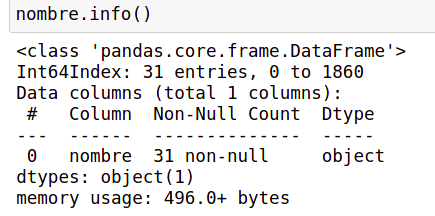
\includegraphics[width=0.5\linewidth]{img/nombre}
  	\caption{}
  	\label{fig:nombre}
  \end{figure}
  
  Por otra parte, para intentar eliminar el ruido que intuimos introduce el algoritmo de SMOTE en el oversampling, vamos a usar otro algoritmo diferente, a saber, SMOTETomek, que combina ambos, oversampling y undersampling, de manera que este último lo que hace es limpiar el ruido que pudo introducir SMOTE. Así, usando SMOTE se lleva a cabo el oversampling y, a continuación, usando lo que se conoce como Tomek Links, se limpia el conjunto resultante. Como \mintinline{python}{sampling_strategy} usamos la de por defecto, de manera que se crean más instancias de todas las clases menos de la mayoritaria. 
  \begin{minted}{python}
  smote=SMOTETomek(random_state=10)
  df_train_over, df_train_obj_over = smote.fit_resample(df_train_num, df_train_obj)
  df_train_over_rpl, df_train_obj_over_rpl = 
  smote.fit_resample(df_train_num_rpl, df_train_obj_replaced)
  Counter(df_train_obj_over)
  
  Counter({1: 1810, 2: 1763, 3: 1716, 4: 1752, 5: 1818})
  \end{minted}
  
  Nos damos cuenta ahora de que no todas las clases tienen el mismo número de instancias, pues se han eliminado algunas usando Tomek Links, como ya hemos comentado, pero las diferencias son muy pequeñas, de manera que el desbalanceo no supondrá un problema. 
  
  El resto de fases del preprocesamiento las aplicamos exactamente de la misma forma que en las útlimas entregas. Así, el proceso de preprocesamiento quedaría como sigue: eliminación de columnas de id y descuento, eliminación de todas las instancias nulas, en los valores del atributo nombre nos quedamos sólo con la primera palabra correspondiente a la marca, normalización de los atributos numéricos, transformación de las variables categóricas a binario usando One-Hot Encoding, oversampling y undersampling con SMOTETomek.
  
  \subsection{Aplicación de los algoritmos}
  Aplicamos los algoritmos que venimos considerando hasta ahora sobre el conjunto de entrenamiento preprocesado de la forma ya descrita, y vemos los valores para la precisión obtenidos usando la función \mintinline{python}{cross_validation}:
  
  \begin{table}[htbp]
  	\caption{}\begin{center}
  	\begin{tabular}{|c|r|r|}
  		\hline
  		\multicolumn{1}{|l|}{} & \multicolumn{1}{l|}{\textbf{Clases desbalanceadas}} & \multicolumn{1}{l|}{\textbf{Oversampling}} \\ \hline
  		LinearSVC & 0.752811 & 0.89943 \\ \hline
  		Knn & 0.748813 & 0.87175 \\ \hline
  		RandomForest & 0.792301 & 0.94486 \\ \hline
  		DecisionTree & 0.743313 & 0.89697 \\ \hline
  		Red Neuronal & 0.755061 & 0.95133 \\ \hline
  		Extra-Trees & 0.774558 & 0.95211 \\ \hline
  		Gradient Boosting & 0.767806 & 0.86304 \\ \hline
  	\end{tabular}\end{center}
  	\label{}
  \end{table}
  
  
  En efecto, los resultados con este preprocesamiento han mejorado con respecto al preprocesamiento anterior, pues mirando la columna de oversampling en el Cuadro 11 de la entrega 8, nos damos cuenta de que allí los resultados son algo inferiores para todos los clasificadores. 
  
  Para esta primera entrega con el nuevo preprocesamiento nos vamos a limitar a entrenar un Random Forest con sus parámetros por defecto, el cual vamos a usar para clasificar el conjunto de test y subir los resultados a Kaggle.
  
  \begin{minted}{python}
  orest=RandomForestClassifier(random_state=10)
  cross_validation(forest, df_train_over,df_train_obj_over,True)
  forest.fit(df_train_over,df_train_obj_over)
  pred=forest.predict(df_test_num)
  ids=df_test_orig["id"]
  
  df_result = pd.DataFrame({'id': ids, 'Precio_cat': pred})
  df_result.to_csv("resultados_14.csv", index=False)
  \end{minted}
  
  \subsection{Características de la entrega}
  
  \begin{table}[htbp]
  	\caption{}\begin{center}
  	\begin{tabular}{|c|c|c|c|c|}
  		\hline
  		\multicolumn{1}{|l|}{\textbf{}} & \textbf{} & \textbf{} & \multicolumn{ 2}{c|}{\textbf{Score}} \\ \hline
  		\textbf{Entrega} & \textbf{Fecha y Hora} & \textbf{Posición en Ranking (hasta ese momento)} & \textbf{Train} & \textbf{Test} \\ \hline
  		\textbf{12} & 27 de diciembre 18:23 & 9 & 0.942136 & 0.70578 \\ \hline
  		\textbf{13} & 27 de diciembre 21:49 & 10 & 0.87889 & 0.73166 \\ \hline
  		\textbf{14} & 28 de diciembre 16:32  & 10 & 0.94875 & 0.74719 \\ \hline
  	\end{tabular}\end{center}
  	\label{}
  \end{table}
  
  Nos damos cuenta entonces de que el resultado obtenido es bastante prometedor, con un simple RandomForest mejoran los resultados obtenidos en las últimas entregas, así que el preprocesamiento considerado para esta entrega es bastante adecuado. Así pues, vamos a seguir usándolo para futuras entregas. 
  \section{Entrega 15}
  \subsection{Preprocesamiento}
  
  El mismo que el realizado para la entrega anterior.
  
  \subsection{Configuración de parámetros}
  
  Nos centramos ahora en el LinearSVC y configuramos su parámetro de regularización C, como hicimos para la entrega 8, con la función \mintinline{python}{tune_svc}, resultando que el mejor valor del mismo es \mintinline{python}{C=50}. EL resto de parámetros o no los hemos considerado o empeoran los resultados al modificarlos, como es el caso de \mintinline{python}{class_weight}
  (el proceso completo está en el notebook \mintinline{python}{p3_10.ipynb})
  
  Entrenamos entonces:
  \begin{minted}{python}
  svc=LinearSVC(random_state=10,C=50,max_iter=100000)
  svc.fit(df_train_over,df_train_obj_over)
  \end{minted}
  
  lo usamos para precedir las clases del conjunto de test y subimos los resultados a Kaggle. 
  
  \subsection{Características de la entrega}

	\begin{table}[htbp]
		\caption{}\begin{center}
		\begin{tabular}{|c|c|c|c|c|}
			\hline
			\multicolumn{1}{|l|}{\textbf{}} & \textbf{} & \textbf{} & \multicolumn{ 2}{c|}{\textbf{Score}} \\ \hline
			\textbf{Entrega} & \textbf{Fecha y Hora} & \textbf{Posición en Ranking (hasta ese momento)} & \textbf{Train} & \textbf{Test} \\ \hline
			\textbf{14} & 28 de diciembre 16:32  & 10 & 0.94875 & 0.74719 \\ \hline
			\textbf{15} & 28 de diciembre 21:33  & 11 & 0.87459 & 0.74201 \\ \hline
		\end{tabular}\end{center}
		\label{}
	\end{table}
	  
	 El resultado obtenido es algo inferior al de RandomForest, pero la diferencia es muy pequeña.
 \section{Entrega 16}
 \subsection{Preprocesamiento}
 El mismo que el realizado en las dos últimas entregas. 
 \subsection{Configuración de parámetros}
 
 Usamos en esta entrega las redes neuronales y configuramos sus parámetros al igual que hicimos para la entrega 6. Para ello usamos la función \mintinline{python}{tune_layers} con un valor máximo de 500, y nos damos cuenta de que el tamaño de capas para el que obtenemos los mejores resultados es (460,460). A continuación, probamos algunos valores aleatorios para el parámetro de regularización alpha, siendo \mintinline{python}{alpha=0.009} el que nos ofrece el valor más alto de la precisión (ver proceso completo en \mintinline{python}{p3_10.ipynb}).
 
 Entrenamos pues la red neuronal con estos parámetros sobre el conjunto de entrenamiento preprocesado y clasificamos el conjunto de test usando la misma:
 
 \begin{minted}{python}
NN=MLPClassifier(hidden_layer_sizes=(460,460),random_state=10,max_iter=10000,alpha=0.009)
cross_validation(NN,df_train_over,df_train_obj_over,True)
NN.fit(df_train_over,df_train_obj_over)
pred=NN.predict(df_test_num)
ids=df_test_orig["id"]

df_result = pd.DataFrame({'id': ids, 'Precio_cat': pred})
df_result.to_csv("resultados_16.csv", index=False)
 \end{minted}
 
 \subsection{Características de la entrega}
 \begin{table}[htbp]
 	\caption{}\begin{center}
 	\begin{tabular}{|c|c|c|c|c|}
 		\hline
 		\multicolumn{1}{|l|}{\textbf{}} & \textbf{} & \textbf{} & \multicolumn{ 2}{c|}{\textbf{Score}} \\ \hline
 		\textbf{Entrega} & \textbf{Fecha y Hora} & \textbf{Posición en Ranking (hasta ese momento)} & \textbf{Train} & \textbf{Test} \\ \hline
 		\textbf{14} & 28 de diciembre 16:32  & 10 & 0.94875 & 0.74719 \\ \hline
 		\textbf{15} & 28 de diciembre 21:33  & 11 & 0.87459 & 0.74201 \\ \hline
 		\textbf{16} & 28 de diciembre 21:53 & 11 & 0.96049 & 0.76272 \\ \hline
 	\end{tabular}\end{center}
 	\label{}
 \end{table}
 
 El resultado ha mejorado notablemente, con lo que la red neuronal es bastante adecuada para llevar a cabo la clasificación. 
 
 \section{Entrega 17}
 \subsection{Preprocesamiento}
 El mismo que hemos llevado a cabo en las tres últimas entregas
 \subsection{Configuración de parámetros}
 Nos quedamos en esta ocasión con Gradient Boosting y configuramos sus parámetros como en la entrega 4. Probando varios valores para el parámetro \mintinline{python}{subsample} llegamos a la conclusión de que el valor más adecuado es 0.8. Para estudiar el parámetro \mintinline{python}{max_depth} empleamos la siguiente función:
 \begin{minted}{python}
 def tune_gradient_boosting(max_value):
	 acc=[]
	 for i in range(2,max_value):
		 gradient=GradientBoostingClassifier(max_depth=i,random_state=10,
		 subsample=0.8)
		 print(i)
		 acc.append(cross_validation(gradient,df_train_over,df_train_obj_over,True))
	 
	 fig, ax =plt.subplots(figsize=(15,5))
	 ax.plot(range(2,max_value), acc)
	 ax.set_title('Gradient Boosting')
	 ax.set_xlabel('Max depth')
	 ax.set_ylabel('Accuracy')
	 plt.show()
 \end{minted}
 
 cuya salida al ejecutarla con un \mintinline{python}{max_value=30} nos lleva a seleccionar como profundidad máxima 19.
 
 Para el número de estimadores consideramos:
 \begin{minted}{python}
def tune_gradient_boosting_2(max_value):
	acc=[]
	for i in range(50,max_value,50):
		gradient=GradientBoostingClassifier(n_estimators=i,max_depth=19,
		random_state=10,subsample=0.8)
		print(i)
		acc.append(cross_validation(gradient,df_train_over,df_train_obj_over,True))
		
	fig, ax =plt.subplots(figsize=(15,5))
	ax.plot(range(50,max_value,50), acc)
	ax.set_title('Gradient Boosting')
	ax.set_xlabel('Num estimadores')
	ax.set_ylabel('Accuracy')
	plt.show()
	
tune_gradient_boosting_2(400)
 \end{minted}
 
 y nos damos cuenta de que la mejor cantidad es \mintinline{python}{n_estimators=100}.
 
 Probando algunos valores para el \mintinline{python}{learning_rate}, vemos que el mejor valor es el de por defecto, esto es, \mintinline{python}{learning_rate=0.1}.
 
 (Ver proceso completo en \mintinline{python}{p3_10.ipynb})
 
 Así pues, tomamos
 \begin{minted}{python}
gradient=GradientBoostingClassifier(learning_rate=0.1,n_estimators=100, random_state=10,
max_features='auto',subsample=0.8,max_depth=19)
 \end{minted}
  y lo entrenamos sobre el conjunto de entrenamiento preprocesado, para después predecir con él las clases de los datos del conjunto de test. 
 
 \subsection{Características de la entrega}
 \begin{table}[htbp]
 	\caption{}\begin{center}
 	\begin{tabular}{|c|c|c|c|c|}
 		\hline
 		\multicolumn{1}{|l|}{\textbf{}} & \textbf{} & \textbf{} & \multicolumn{ 2}{c|}{\textbf{Score}} \\ \hline
 		\textbf{Entrega} & \textbf{Fecha y Hora} & \textbf{Posición en Ranking (hasta ese momento)} & \textbf{Train} & \textbf{Test} \\ \hline
 		\textbf{14} & 28 de diciembre 16:32  & 10 & 0.94875 & 0.74719 \\ \hline
 		\textbf{15} & 28 de diciembre 21:33  & 11 & 0.87459 & 0.74201 \\ \hline
 		\textbf{16} & 28 de diciembre 21:53 & 11 & 0.96049 & 0.76272 \\ \hline
 		\textbf{17} & 29 de diciembre 20:12 & 12 & 0.94401 & 0.7748 \\ \hline
 	\end{tabular}\end{center}
 	\label{}
 \end{table}
 
 Es claro entonces que, de los clasificadores considerados hasta el momento, este es el que ha dado un mejor resultado al clasificar las instancias del conjunto de test.
 
 \section{Entregas 18 y 19}
 \subsection{Preprocesamiento}
 El mismo que el llevado a cabo para la entrega anterior.
 \subsection{Aplicación de los algoritmos}
 Una vez que tenemos los parámetros de algunos de los mejores clasificadores configurados y sabemos que nos dan resultados aceptables en Kaggle, vamos a proceder a realizar Stacking de algunos de ellos para estas entregas. De las opciones probadas, la que ofrece un valor mayor de la precisión usando la función \mintinline{python}{cross-validation} es la siguiente:
 \begin{minted}{python}
 forest=RandomForestClassifier(random_state=10)
 svc=LinearSVC(random_state=10,C=50,max_iter=100000)
 NN=MLPClassifier(hidden_layer_sizes=(460,460),random_state=10,max_iter=10000,alpha=0.009)
 gradient=GradientBoostingClassifier(n_estimators=100, random_state=10,max_features='auto',
 subsample=0.8,max_depth=19)
 
 estimators = [('Linear SVC', svc),
 ('forest', forest),('gradient', gradient),('Red',NN)]
 
 clf = StackingClassifier(estimators=estimators, final_estimator=gradient,cv=5)
 cross_validation(clf, df_train_over, df_train_obj_over,True)
 
 Accuracy:  0.9647835774001248
 \end{minted}
 
 por lo que lo vamos a usar para la Entrega 18. 
 
 La siguiente configuración que presenta el mejor resultado es igual a la anterior pero cambiando el estimador final por RandomForest:
 
 \begin{minted}{python}
 estimators = [('Linear SVC', svc),
 ('forest', forest),('gradient', gradient),('Red',NN)]
 
 clf = StackingClassifier(estimators=estimators, final_estimator=forest,cv=5)
 cross_validation(clf, df_train_over, df_train_obj_over,True)
 
 Accuracy:  0.9636549729591245
 \end{minted}
  
  Usaremos este clasificador para la Entrega 19. 
  \newpage
  \subsection{Características de las entregas}
  \begin{table}[htbp]
  	\caption{}\begin{center}
  	\begin{tabular}{|c|c|c|c|c|}
  		\hline
  		\multicolumn{1}{|l|}{\textbf{}} & \textbf{} & \textbf{} & \multicolumn{ 2}{c|}{\textbf{Score}} \\ \hline
  		\textbf{Entrega} & \textbf{Fecha y Hora} & \textbf{Posición en Ranking (hasta ese momento)} & \textbf{Train} & \textbf{Test} \\ \hline
  		\textbf{14} & 28 de diciembre 16:32  & 10 & 0.94875 & 0.74719 \\ \hline
  		\textbf{15} & 28 de diciembre 21:33  & 11 & 0.87459 & 0.74201 \\ \hline
  		\textbf{16} & 28 de diciembre 21:53 & 11 & 0.96049 & 0.76272 \\ \hline
  		\textbf{17} & 29 de diciembre 20:12 & 12 & 0.94401 & 0.7748 \\ \hline
  		\textbf{18} & 29 de diciembre 23:35  & 13 & 0.964783 & 0.75754 \\ \hline
  		\textbf{19} & 30 de diciembre 00:42  & 13 & 0.963654 & 0.77135 \\ \hline
  	\end{tabular}\end{center}
  	\label{}
  \end{table}
  
  Nos damos cuenta de que en este caso la estrategia de Stacking no ha mejorado los resultados, sino que incluso ha empeorado el resultado que obtuvimos con GradientBoosting en la entrega 17. 
  
  \section{Entrega 20}
  \subsection{Preprocesamiento}
  El mismo que hemos realizado para la entrega anterior
  \subsection{Configuración de los parámetros}
  Vamos a configurar los parámetros del clasificador de Extra-Trees de la misma forma que lo hicimos para la entrega 12. Para la opción de Bootstrap obtenemos un mejor resultado con la misma desactivada. Para el número de estimadores usamos la función \mintinline{python}{tune_num_arboles} de igual manera que en la entrega 12 y vemos que para \mintinline{python}{n_estimators=180} la precisión es lo mejor posible. Cambiar el parámetro \mintinline{python}{max_depth} solo empeora los resultados, por lo que este lo dejamos con la opción por defecto. (Ver los detalles en el notebook \mintinline{python}{p3_11.ipynb})
  
  Así, usaremos \mint{python}{extra=ExtraTreesClassifier(n_estimators=180,random_state=10)} que nos ofrece 
   \mintinline{python}{Accuracy:  0.9550761}.
  \subsection{Aplicación de los algoritmos}
  Para intentar mejorar los resultados proporcionados por los Stackings realizados para las entregas anteriores, vamos a incluir en los estimadores el clasificador de Extra-Trees, pues este era el que presentaba el valor más alto de la precisión en el Cuadro 18 de la entrega 15 para el preprocesamiento que estamos considerando:
  
  \begin{minted}{python}
  estimators = [('Linear SVC', svc),
  ('forest', forest),('gradient', gradient),('Red',NN),('extra',extra)]
  
  clf = StackingClassifier(estimators=estimators, final_estimator=forest,cv=5)
  cross_validation(clf, df_train_over, df_train_obj_over,True)
  
  Accuracy: 0.9653479114859035
  \end{minted}
  
  Vemos que de hecho la precisión ha aumentado un poco con respecto a la obtenida con los Stackings de las dos entregas anteriores. Entrenamos por tanto este clasificador sobre el conjunto de entrenamiento preprocesado, predecimos con él las clases de los datos del conjunto de test y subimos los resultados. 
  
  \subsection{Características de la entrega}
  \begin{table}[htbp]
  	\caption{}
  	\begin{tabular}{|c|c|c|c|c|}
  		\hline
  		\multicolumn{1}{|l|}{\textbf{}} & \textbf{} & \textbf{} & \multicolumn{ 2}{c|}{\textbf{Score}} \\ \hline
  		\textbf{Entrega} & \textbf{Fecha y Hora} & \textbf{Posición en Ranking (hasta ese momento)} & \textbf{Train} & \textbf{Test} \\ \hline
  		\textbf{14} & 28 de diciembre 16:32  & 10 & 0.94875 & 0.74719 \\ \hline
  		\textbf{15} & 28 de diciembre 21:33  & 11 & 0.87459 & 0.74201 \\ \hline
  		\textbf{16} & 28 de diciembre 21:53 & 11 & 0.96049 & 0.76272 \\ \hline
  		\textbf{17} & 29 de diciembre 20:12 & 12 & 0.94401 & 0.7748 \\ \hline
  		\textbf{18} & 29 de diciembre 23:35  & 13 & 0.964783 & 0.75754 \\ \hline
  		\textbf{19} & 30 de diciembre 00:42  & 13 & 0.963654 & 0.77135 \\ \hline
  		\textbf{20} & 30 de diciembre 16:29  & 15 & 0.965347 & 0.75841 \\ \hline
  	\end{tabular}
  	\label{}
  \end{table}
  
  El resultado ha bajado considerablemente con respecto a la entrega anterior, lo que indica que quizás este clasificador sea peor de lo que parece, pues ha influido negativamente en el stacking. 
  
  \section{Entregas 21 y 22}
  \subsection{Preprocesamiento}
  
  Viendo que no hay manera de mejorar los resultados ni con stacking de los mejores clasificadores con sus parámetros configurados, vamos a volver al preprocesamiento que llevamos a cabo para las entregas 11 y 12, esto es: eliminación de columnas de id y descuento, eliminació de todas las instancias nulas, normalización de los atributos numéricos, transformación de las variables categóricas a binario usando One-Hot
  Encoding y Oversampling con el algoritmo de SMOTE con parámetros por defecto. 
  
  El código se encuentra en el mismo notebook que la entrega 12, es decir, en \mintinline{python}{p3_8.ipynb}
  
  Nos centraremos en configurar los parámetros de los algoritmos que nos vienen dando los mejores resultados hasta ahora. 
  \subsection{Configuración de parámetros}
  \subsubsection{Redes Neuronales}
  Configuramos el tamaño de las capas y el parámetro de regularización alpha como hicimos para la entrega 16, usando la función \mintinline{python}{tune_layers} y después probando distintos valores para alpha. De esta manera, los mejores resultados los hemos obtenido para un tamaño de capas de (340,340) y \mintinline{python}{alpha=0.05}. Así, consideramos 
  \begin{minted}{python}
  NN=MLPClassifier(hidden_layer_sizes=(340,340),random_state=10,max_iter=10000,alpha=0.05)
  cross_validation(NN,df_train_over,df_train_obj_over,True)
  
  Accuracy:  0.9529863013698631
  \end{minted}
   y lo usamos para la \underline{entrega 21}.
  
  \subsubsection{Gradient Boosting}
  
  Para este clasificador, configuramos como venimos haciendo hasta ahora los parámetros \mintinline{python}{subsample,learning_rate,max_depth,n_estimators}, usando las funciones \mintinline{python}{tune_gradient_boosting} para la profundidad máxima y \mintinline{python}{tune_gradient_boosting_2} para el número de estimadores, funciones cuyo código ya usamos para la entrega 17, y probando distintos valores para los parámetros \mintinline{python}{subsample} y \mintinline{python}{learning_rate}. Llegamos de esta forma a que la mejor configuración para los parámetros es la siguiente:
  
  \begin{minted}{python}
  gradient=GradientBoostingClassifier(n_estimators=400, learning_rate=0.1, random_state=10,
  max_features='auto',subsample=0.8,max_depth=16)
  cross_validation(gradient,df_train_over,df_train_obj_over,True)
  
  Accuracy:  0.9461594054193917
  \end{minted}
  
  de manera que vamos a usar Gradient Boosting con esta configuración de parámetros para clasificar el conjunto de test y realizar la \underline{entrega 22} 
  \subsection{Características de las entregas}
  
  \begin{table}[htbp]
  	\caption{}\begin{center}
  	\begin{tabular}{|c|c|c|c|c|}
  		\hline
  		\multicolumn{1}{|l|}{\textbf{}} & \textbf{} & \textbf{} & \multicolumn{ 2}{c|}{\textbf{Score}} \\ \hline
  		\textbf{Entrega} & \textbf{Fecha y Hora} & \textbf{Posición en Ranking (hasta ese momento)} & \textbf{Train} & \textbf{Test} \\ \hline
  		\textbf{14} & 28 de diciembre 16:32  & 10 & 0.94875 & 0.74719 \\ \hline
  		\textbf{15} & 28 de diciembre 21:33  & 11 & 0.87459 & 0.74201 \\ \hline
  		\textbf{16} & 28 de diciembre 21:53 & 11 & 0.96049 & 0.76272 \\ \hline
  		\textbf{17} & 29 de diciembre 20:12 & 12 & 0.94401 & 0.7748 \\ \hline
  		\textbf{18} & 29 de diciembre 23:35  & 13 & 0.964783 & 0.75754 \\ \hline
  		\textbf{19} & 30 de diciembre 00:42  & 13 & 0.963654 & 0.77135 \\ \hline
  		\textbf{20} & 30 de diciembre 16:29  & 15 & 0.965347 & 0.75841 \\ \hline
  		\textbf{21} & 30 de diciembre 16:50 & 15 & 0.95298 & 0.76186 \\ \hline
  		\textbf{22} & 30 de diciembre 23:34 & 19 & 0.946159 & 0.74374 \\ \hline
  	\end{tabular}\end{center}
  	\label{}
  \end{table}

La red neuronal (entrega 21) ofrece buenos resultados, pero no son mejores que los obtenidos para la misma en la entrega 16, donde la entrenamos con datos preprocesados usando oversampling con SMOTETomek y eliminando detalles del atributo nombre. Lo mismo ocurre para el algoritmo de Gradient Boosting (entrega 22), donde de hecho el resultado ha bajado considerablemente con respecto a la entrega 17, en la que también usamos Gradient Boosting con los datos preprocesados como en la entrega 16. Así pues, no merece la pena seguir con el preprocesamiento que hemos considerado aquí para las entregas y vamos a probar algo difente. 
  
  
\section{Entrega 23}
  \subsection{Preprocesamiento}
  Para esta última entrega cambiamos de nuevo el preprocesamiento. Esta vez vamos a usar LabelEncoder para tratar las variables categóricas en lugar de One-Hot Encoding, y vamos a aplicar oversampling con un algoritmo diferente, esto es, con Borderline SMOTE, que es una variante del algoritmo de SMOTE.  Además, como hicimos para las entregas 14 a la 20, en el atributo de nombre nos vamos a quedar simplemente con la marca del coche. 
  
  Por lo tanto, los pasos seguidos en el preprocesamiento han sido los siguientes:
 \begin{enumerate}
  	\item Eliminación de columnas de id y descuento
  	\item  Eliminación de todas las instancias nulas
  	\item  En los valores del atributo nombre nos quedamos sólo con la primera palabra correspondiente a la marca
  	\item  Transformamos las variables categóricas a numéricas usando LabelEncoder
  	\item  Normalización de todos los datos
  	\item  Oversampling usando el algoritmo BorderlineSMOTE con parámetros por defecto
  \end{enumerate}
  
  \subsection{Aplicación de los algoritmos}
  Nos vamos a centrar en el algoritmo de Gradient Boosting, pues ha sido el clasificador que nos ha proporcionado los mejores resultados en Kaggle para casi todos los preprocesamientos que hemos considerado. Así pues, configuramos sus parámetros y lo entrenamos con el conjunto de entrenamiento con este nuevo preprocesamiento. 
  \subsubsection{Configuración de los parámetros}
  Como ya hemos hecho en las entregas 4, 17 y 22, analizamos los parámetros \mintinline{python}{subsample,learning_rate,} \mintinline{python}{max_depth, n_estimators} de Gradient Boosting. Para ello procedemos exactamente de la misma forma que en dichas entregas y llegamos a que los valores de los parámetros que nos ofrecen las precisiones más altas son los siguientes:
  \begin{minted}{python}
  gradient=GradientBoostingClassifier(n_estimators=450, learning_rate=0.1, random_state=10,
  max_features='auto',subsample=0.5,max_depth=8)
  \end{minted}
  
  y tras correr la función \mint{python}{cross_validation(gradient,df_train_over,df_train_obj_over,True)} obtenemos \mintinline{python}{Accuracy:  0.9117808219178082}
  \newpage
  \subsection{Características de la entrega}
  
  \begin{table}[htbp]
  	\caption{}\begin{center}
  	\begin{tabular}{|c|c|c|c|c|}
  		\hline
  		\multicolumn{1}{|l|}{\textbf{}} & \textbf{} & \textbf{} & \multicolumn{ 2}{c|}{\textbf{Score}} \\ \hline
  		\textbf{Entrega} & \textbf{Fecha y Hora} & \textbf{Posición en Ranking (hasta ese momento)} & \textbf{Train} & \textbf{Test} \\ \hline
  		\textbf{17} & 29 de diciembre 20:12 & 12 & 0.94401 & 0.7748 \\ \hline
  		\textbf{18} & 29 de diciembre 23:35  & 13 & 0.964783 & 0.75754 \\ \hline
  		\textbf{19} & 30 de diciembre 00:42  & 13 & 0.963654 & 0.77135 \\ \hline
  		\textbf{20} & 30 de diciembre 16:29  & 15 & 0.965347 & 0.75841 \\ \hline
  		\textbf{21} & 30 de diciembre 16:50 & 15 & 0.95298 & 0.76186 \\ \hline
  		\textbf{22} & 30 de diciembre 23:34 & 19 & 0.946159 & 0.74374 \\ \hline
  		\textbf{23} & 31 de diciembre 16:18 & 21 & 0.91178 & 0.7515 \\ \hline
  	\end{tabular}\end{center}
  	\label{}
  \end{table}

El resultado ha mejorado con respecto a la última entrega, en que también usamos Gradient Boosting pero con datos con un preprocesamiento diferente, pero no lo ha hecho con respecto a la entrega 17, donde este ofrecía el mejor resultado para Gradient Boosting de todos los preprocesamientos realizados. 
  \section{Conclusiones}
Una vez cerrada la competición, revisando mis subidas y pasos seguidos y escribiendo la memoria, me he dado cuenta de muchos detalles que no he tenido en cuenta y que podrían ser el motivo de no haber conseguido mejorar. 

Empecé a probar cosas de manera bastante organizada y lógica, al menos a mi parecer, pero conforme avanzaban los días y las pruebas que realizaba, sentía que nada conseguía mejorar los resultados. Comencé a frustrarme y a probar cosas a lo loco, y el estrés y la ansiedad se apoderaron de mí. Entonces empezó la desorganización, el bloqueo y el ignorar detalles importantes. Nótese el desorden en las entregas finales. 

En primer lugar, lo más importante de todo, que no tuve en cuenta y que podría haber sido de gran ayuda, es que realicé la validación sobre el conjunto de entrenamiento tras realizar el oversampling o undersampling. Lo mejor habría sido dejar una parte del conjunto original, sobre la que no aplicaría la técnica de oversampling ni undersampling (según el caso), y validar los resultados sobre dicha parte del conjunto, dejando una parte diferente cada vez según la técnica de la validación cruzada. De esta forma, el conjunto de validación habría sido más parecido al conjunto de test, en el que no se han creado instancias nuevas con oversampling o eliminado otras con undersampling, y los valores de la precisión habrían sido más parecidos a los que se obtendrían sobre el conjunto de test. Así, a la hora de configurar los parámetros y decidir qué clasificadores eran mejores, los valores de la precisión sobre el conjunto de entrenamiento que han servido de guía serían más adecuados y la elección habría sido mejor. 

Por otra parte, al llevar a cabo Stacking de varios clasificadores, el incluir algún clasificador con un resultado más bajo hizo que los resultados proporcionados por el mismo fueran algo peores. En su lugar, debería haber probado incluyendo menos clasificadores en el Stacking y solamente aquellos con un buen valor de la precisión. 

Además, revisando el código, me di cuenta de otras configuraciones de parámetros que proporcionaban mejores resultados, y de opciones de Stacking mejores. También debería haber configurado los parámetros en conjunto, y no de manera individual cada uno de ellos como yo he hecho. 
 
\textbf{Nota:} Al correr el código de nuevo, para dejar los notebooks organizados y presentables, los resultados han variado ligeramente con respecto a los que obtuve en el momento de realizar las entregas y configurar los parámetros. Por eso, si se miran las salidas ahora, puede que haya otros valores de los parámetros para los que la precisión sea más alta a los que yo consideré para la entrega (y que he incluido en la memoria), y los valores de la precisión sobre el conjunto de entrenamiento de las entregas finales también pueden variar con respecto a los que obtuve en su momento, que son los que he considerado a la hora de escribir la memoria.  
  \section{Tabla resumen de las subidas}
  
  \begin{table}[htbp]
  	\caption{}\begin{center}
  	\begin{tabular}{|c|c|c|c|c|c|}
  		\hline
  		\textbf{} & \textbf{} & \textbf{} & \multicolumn{ 2}{c|}{\textbf{Score}} & \multicolumn{1}{l|}{} \\ \hline
  		\textbf{Entrega} & \textbf{Fecha y Hora} & \textbf{Posición en Ranking} & \textbf{Train} & \textbf{Test} & \textbf{Código} \\ \hline
  		\textbf{1} & 23 de diciembre 21:30 & 10 & 0.822526 & 0.74374 & P3\_1 \\ \hline
  		\textbf{2} & 24 de diciembre 16:51 & 10 & 0.824541 & 0.74029 & P3\_2 \\ \hline
  		\textbf{3} & 24 de dic iembre19:49 & 13 & 0.810294 & 0.72389 & P3\_3 \\ \hline
  		\textbf{4} & 24 de diciembre 21:00 & 7 & 0.836037 & 0.76704 & P3\_3 \\ \hline
  		\textbf{5} & 25 de diciembre 13:07 & 7 & 0.814792 & 0.73856 & P3\_4 \\ \hline
  		\textbf{6} & 25 de diciembre 19:10 & 7 & 0.757802 & 0.69801 & P3\_5 \\ \hline
  		\textbf{7} & 25 de diciembre 19:24 & 7 & 0.835037 & 0.77308 & P3\_6 \\ \hline
  		\textbf{8} & 26 de diciembre 20:04 & 9 & 0.957309 & 0.61087 & P3\_7 \\ \hline
  		\textbf{9} & 26 de diciembre 20:06 & 9 & 0.957309 & 0.61259 & P3\_7 \\ \hline
  		\textbf{10} & 26 de diciembre 23:03 & 9 & 0.971929 & 0.62295 & P3\_7 \\ \hline
  		\textbf{11} & 27 de diciembre  17:43 & 9 & 0.9524383 & 0.71786 & P3\_7 \\ \hline
  		\textbf{12} & 27 de diciembre 18:23 & 9 & 0.942136 & 0.70578 & P3\_8 \\ \hline
  		\textbf{13} & 27 de diciembre 21:49 & 10 & 0.87889 & 0.73166 & P3\_9 \\ \hline
  		\textbf{14} & 28 de diciembre 16:32  & 10 & 0.94875 & 0.74719 & P3\_10 \\ \hline
  		\textbf{15} & 28 de diciembre 21:33  & 11 & 0.87459 & 0.74201 & P3\_10 \\ \hline
  		\textbf{16} & 28 de diciembre 21:53 & 11 & 0.96049 & 0.76272 & P3\_10 \\ \hline
  		\textbf{17} & 29 de diciembre 20:12 & 12 & 0.94401 & 0.7748 & P3\_10 \\ \hline
  		\textbf{18} & 29 de diciembre 23:35  & 13 & 0.964783 & 0.75754 & P3\_11 \\ \hline
  		\textbf{19} & 30 de diciembre 00:42  & 13 & 0.963654 & 0.77135 & P3\_11 \\ \hline
  		\textbf{20} & 30 de diciembre 16:29  & 15 & 0.965347 & 0.75841 & P3\_11 \\ \hline
  		\textbf{21} & 30 de diciembre 16:50 & 15 & 0.95298 & 0.76186 & P3\_8 \\ \hline
  		\textbf{22} & 30 de diciembre 23:34 & 19 & 0.946159 & 0.74374 & P3\_8 \\ \hline
  		\textbf{23} & 31 de diciembre 16:18 & 21 & 0.91178 & 0.7515 & P3\_12 \\ \hline
  	\end{tabular}\end{center}
  	\label{}
  \end{table}
  
  La columna de Código indica el nombre del notebook de Jupyter donde se encuentra el código correspondiente a cada entrega. 

  
\newpage
\begin{thebibliography}{9}
\bibitem{1} 	
\url{https://scikit-learn.org/stable/modules/generated/sklearn.preprocessing.OneHotEncoder.html}

\bibitem{2} 
\url{https://www.analyticsvidhya.com/blog/2020/03/one-hot--vs-label-encoding-using-scencodingikit-learn/}

\bibitem{3} 
\url{https://imbalanced-learn.readthedocs.io/en/stable/generated/imblearn.over_sampling.SMOTE.html}

\bibitem{4} 
\url{https://imbalanced-learn.readthedocs.io/en/stable/generated/imblearn.under_sampling.EditedNearestNeighbours.html#imblearn.under_sampling.EditedNearestNeighbours}

\bibitem{5} 
\url{https://imbalanced-learn.readthedocs.io/en/stable/under_sampling.html}
\bibitem{6} 
\url{https://imbalanced-learn.readthedocs.io/en/stable/over_sampling.html}
\bibitem{7} 
\url{https://scikit-learn.org/stable/modules/generated/sklearn.ensemble.ExtraTreesClassifier.html}
\bibitem{8} 
\url{https://scikit-learn.org/stable/modules/generated/sklearn.ensemble.BaggingClassifier.html}
\bibitem{9} 
\url{https://scikit-learn.org/stable/modules/generated/sklearn.neural_network.MLPClassifier.html#sklearn.neural_network.MLPClassifier}
\bibitem{10} 
\url{https://scikit-learn.org/stable/modules/generated/sklearn.ensemble.GradientBoostingClassifier.html}
\bibitem{11} 
\url{https://scikit-learn.org/stable/modules/generated/sklearn.svm.LinearSVC.html}
\bibitem{12} 
\url{https://scikit-learn.org/stable/modules/generated/sklearn.ensemble.AdaBoostClassifier.html}
\bibitem{13}
\url{https://scikit-learn.org/stable/modules/generated/sklearn.ensemble.StackingClassifier.html}
\bibitem{14}
\url{https://imbalanced-learn.readthedocs.io/en/stable/generated/imblearn.over_sampling.BorderlineSMOTE.html}
\bibitem{15}
\url{https://imbalanced-learn.readthedocs.io/en/stable/generated/imblearn.combine.SMOTETomek.html#imblearn.combine.SMOTETomek}
\bibitem{16}
\url{https://scikit-learn.org/stable/modules/generated/sklearn.ensemble.RandomForestClassifier.html}

\end{thebibliography}
\end{document}
